\documentclass[11pt,a4paper]{article}

\usepackage[T1]{fontenc}
\usepackage[utf8]{inputenc}
\usepackage{lmodern}
\usepackage{microtype}
\usepackage[a4paper,margin=2.25cm,headheight=15pt]{geometry}
\usepackage{amsmath,amssymb,mathtools}
\usepackage{booktabs,tabularx,array,longtable}
\usepackage{graphicx}
\usepackage{xcolor}
\usepackage{caption}
\usepackage{subcaption}
\usepackage{enumitem}
\usepackage{fancyhdr}
\usepackage{placeins}
\usepackage{hyperref}

\definecolor{navy}{HTML}{102A43}
\definecolor{blue}{HTML}{1769E0}
\definecolor{cyan}{HTML}{00A6A6}
\definecolor{green}{HTML}{168B5B}
\definecolor{purple}{HTML}{7A5AF8}
\definecolor{orange}{HTML}{F28E2B}
\definecolor{muted}{HTML}{66788A}
\definecolor{light}{HTML}{F3F6F9}

\hypersetup{colorlinks=true,linkcolor=navy,citecolor=purple,urlcolor=blue,
  pdftitle={Designing the Boundary: Constitutive Markov-Blanket Inversion in Individual and Collective Drones},
  pdfauthor={Luca M. Possati},
  pdfkeywords={active inference, Markov blanket, design theory, collective agency}}
\graphicspath{{../results/}{../results/extended/}{../collective_results/}{results/}{results/extended/}{collective_results/}}
\pagestyle{fancy}
\fancyhf{}
\lhead{\textcolor{muted}{The Boundary-Designing Drone}}
\rhead{\textcolor{muted}{Individual and collective boundary design}}
\cfoot{\thepage}
\renewcommand{\headrulewidth}{0.4pt}
\numberwithin{equation}{section}
\setlength{\parindent}{0pt}
\setlength{\parskip}{0.52em}
\setlist[itemize]{leftmargin=1.45em,itemsep=0.2em,topsep=0.3em}
\captionsetup{font=small,labelfont=bf}

\newcommand{\Irole}{\mathsf{I}}
\newcommand{\Srole}{\mathsf{S}}
\newcommand{\Arole}{\mathsf{A}}
\newcommand{\Erole}{\mathsf{E}}
\newcommand{\KL}{D_{\mathrm{KL}}}
\newcommand{\indep}{\perp\!\!\!\perp}
\newcommand{\Hent}{\mathrm{H}}
\newcommand{\MI}{\mathrm{I}}
\newcommand{\E}{\mathbb{E}}
\newcommand{\R}{\mathbb{R}}
\newcommand{\Mset}{\mathcal{M}}
\newcommand{\Corg}{\mathcal{C}}
\newcommand{\Tmap}{\mathcal{T}}
\newcommand{\Gap}{\Delta_{\mathrm{fac}}}

\newenvironment{keybox}{\begin{center}\begin{minipage}{0.94\textwidth}\color{navy}\hrule\vspace{0.55em}\small}
  {\vspace{0.55em}\hrule\end{minipage}\end{center}}

\IfFileExists{results_macros.tex}{\newcommand{\NSeeds}{20}
\newcommand{\NTotal}{360}
\newcommand{\ConstructFull}{95}
\newcommand{\ConstructDiag}{0}
\newcommand{\StabilizeFull}{95}
\newcommand{\StabilizeDiag}{0}
\newcommand{\TransformFull}{100}
\newcommand{\TransformDiag}{0}
\newcommand{\ConstructGapDelta}{$-26.57\pm0.86$}
\newcommand{\StabilizeGapDelta}{$-8.23\pm0.60$}
\newcommand{\TransformViabilityDelta}{$+0.090\pm0.005$}
\newcommand{\ArchitectureIndirect}{0.508}
\newcommand{\ArchitectureIndirectLow}{0.313}
\newcommand{\ArchitectureIndirectHigh}{0.760}
}{
  \newcommand{\NSeeds}{20}
  \newcommand{\NTotal}{360}
  \newcommand{\ConstructFull}{--}
  \newcommand{\ConstructDiag}{--}
  \newcommand{\StabilizeFull}{--}
  \newcommand{\StabilizeDiag}{--}
  \newcommand{\TransformFull}{--}
  \newcommand{\TransformDiag}{--}
  \newcommand{\ConstructGapDelta}{--}
  \newcommand{\StabilizeGapDelta}{--}
  \newcommand{\TransformViabilityDelta}{--}
  \newcommand{\ArchitectureIndirect}{--}
  \newcommand{\ArchitectureIndirectLow}{--}
  \newcommand{\ArchitectureIndirectHigh}{--}
}

\title{\vspace{-1.1cm}{\color{navy}\LARGE\bfseries Designing the Boundary}\\[0.35em]
  {\large Constitutive Markov-Blanket Inversion in Individual\\
  and Collective Drones}}
\author{Luca M. Possati}
\date{September 2026}

\begin{document}
\maketitle

\begin{abstract}
Active-inference models usually assume the Markov blanket through which an
agent senses and acts. This paper asks a stronger design-theoretic question:
can an artifact infer all four blanket roles and then select interventions
that make a different boundary empirically true? The physical causal
organization, $\Corg_t$, is separated from the artifact's posterior belief
about that organization, $q_t(M)$. Each drone maintains an exact joint
posterior over all $8!/(2!)^4=2520$ assignments of eight modules to internal,
sensory, active, and external roles; learns transition and intervention
models online; and selects control and design actions as a joint policy by
expected free energy (EFE). Shielding removes unscreened interior--exterior
drift channels, while routing exchanges the physical modules occupying causal
ports. The intervention is therefore constitutive rather than merely
diagnostic.

The paper has two experimental parts. Part~I tests an individual drone on the
three verbs central to Possati's \emph{Design for Entropy}: construct,
stabilize, and transform. Across 360 frozen missions, the constitutive agent
succeeds in \ConstructFull\%, \StabilizeFull\%, and \TransformFull\% of the
respective tasks, versus \ConstructDiag\%, \StabilizeDiag\%, and
\TransformDiag\% for a diagnostic-only control. Part~II asks whether two
drones can infer and enact a group-level blanket. No unilateral proposal can
change the group organization; evidence pooling and a bilateral EFE
handshake are required. Across 420 additional missions, the collective agent
succeeds in 80\% of assembly trials, 90\% of repair trials, and 100\% of
reconfiguration trials. An equal-bandwidth communication control succeeds in
0\% of all three. These results establish a bounded proof of concept for
causal boundary design and operational collective individuation. They do not
establish open-ended self-individuation, hardware autonomy, or the ontological
identity of a drone swarm.
\end{abstract}

\noindent\textbf{Keywords:} active inference; Markov blanket; expected free
energy; design theory; structural learning; path space; causal intervention;
collective agency; multi-agent systems.

{\small\tableofcontents}
\newpage

\section{Introduction}

Autonomous systems normally learn inside an interface that engineers have
already fixed. Sensors are inputs, motors are outputs, software variables are
internal, and everything else is environment. Parameters may change, but the
partition that makes those parameters meaningful is treated as invariant.
This assumption is fragile whenever channels fail, resources are rerouted, or
the task requires a different coupling between artifact and world.

The free-energy principle (FEP) and active inference provide a statistical
vocabulary for questioning that assumption. An adaptive system can be
described by exterior states $Y$, interior states $X$, and boundary states
$B=(S,A)$, where sensory states $S$ mediate exterior influence on the
interior and active states $A$ mediate interior influence on the exterior
\cite{friston2009,friston2010,kirchhoff2018,friston2019,ramstead2023}. At an
instant, a Markov blanket satisfies
\begin{equation}
  Y_t\indep X_t\mid B_t.
  \label{eq:fixed-blanket}
\end{equation}
The stronger path-space statement is
\begin{equation}
  Y_{[0,T]}\indep X_{[0,T]}\mid B_{[0,T]},
  \label{eq:path-blanket}
\end{equation}
which rules out hidden temporal channels that an instantaneous graph can miss
\cite{friston2023,sakthivadivel2026}.

Beck and Ramstead treat blanket identification as generative-model inversion:
the system infers which microscopic variables occupy macroscopic functional
roles from their dynamics \cite{beckramstead2025}. Possati's proposal in
\emph{Design for Entropy} reverses the practical direction of that inversion
\cite{possati2026}. If model inversion can disclose a statistical boundary,
design can select interventions that construct, stabilize, or transform the
couplings that make a boundary true. The reversal is not a change of label.
It changes the object of action from a belief about organization to the
organization itself.

This distinction yields two nested research questions:
\begin{keybox}
\textbf{RQ1---individual constitution.} Can a computational artifact jointly infer all
four roles of its Markov-blanket organization, learn how structural
interventions work, and use EFE to select control and design actions that
\emph{cause} a path-space boundary to be constructed, stabilized, or
transformed---with measurable consequences for viability?

\textbf{RQ2---collective constitution.} Can two partially informed artifacts
pool structural evidence and jointly enact a group-level boundary that no
member can constitute alone, and does that boundary improve their strategic
performance relative to individual, fixed-team, random, and equal-bandwidth
communication controls?
\end{keybox}

The question is deliberately discriminating. A model does not count as
boundary design merely because its estimate $q_t(M)$ changes. It counts only
if a chosen design action $d_t$ changes the physical causal organization:
\begin{equation}
  \frac{\partial \Corg_{t+1}}{\partial d_t}\ne 0,
  \label{eq:discriminating}
\end{equation}
or, for discrete actions, if two admissible actions under the same exogenous
realization produce different $\Corg_{t+1}$.
This interventionist criterion follows the ordinary causal distinction
between observing a variable and changing the mechanism that generates it
\cite{pearl2009,peters2017}.

The contribution is fourfold. First, the model separates epistemic boundary
beliefs from the physical causal organization on which those beliefs bear.
Second, it makes discovery complete: internal, sensory, active, and external
roles are inferred jointly as a constrained partition, rather than treating
one role as an unexamined anchor. Third, it learns intervention efficacy and
selects motor and structural actions in one EFE policy. Fourth, it extends
boundary design across scale: a pair of drones must establish a shared
blanket through evidence pooling and bilateral agreement.

The paper proceeds from the common conceptual framework to two experimental
parts. Sections~2--3 introduce the FEP, active inference, and Possati's
design-theoretic inversion. Part~I specifies and tests individual boundary
design. Part~II defines a genuinely joint boundary and tests its strategic
value. The discussion separates computational evidence for operational
individuation from stronger metaphysical claims. Appendices provide the
path-space derivation, algorithms, parameter register, complete result
tables, and reproducibility information.

\begin{figure}[t]
  \centering
  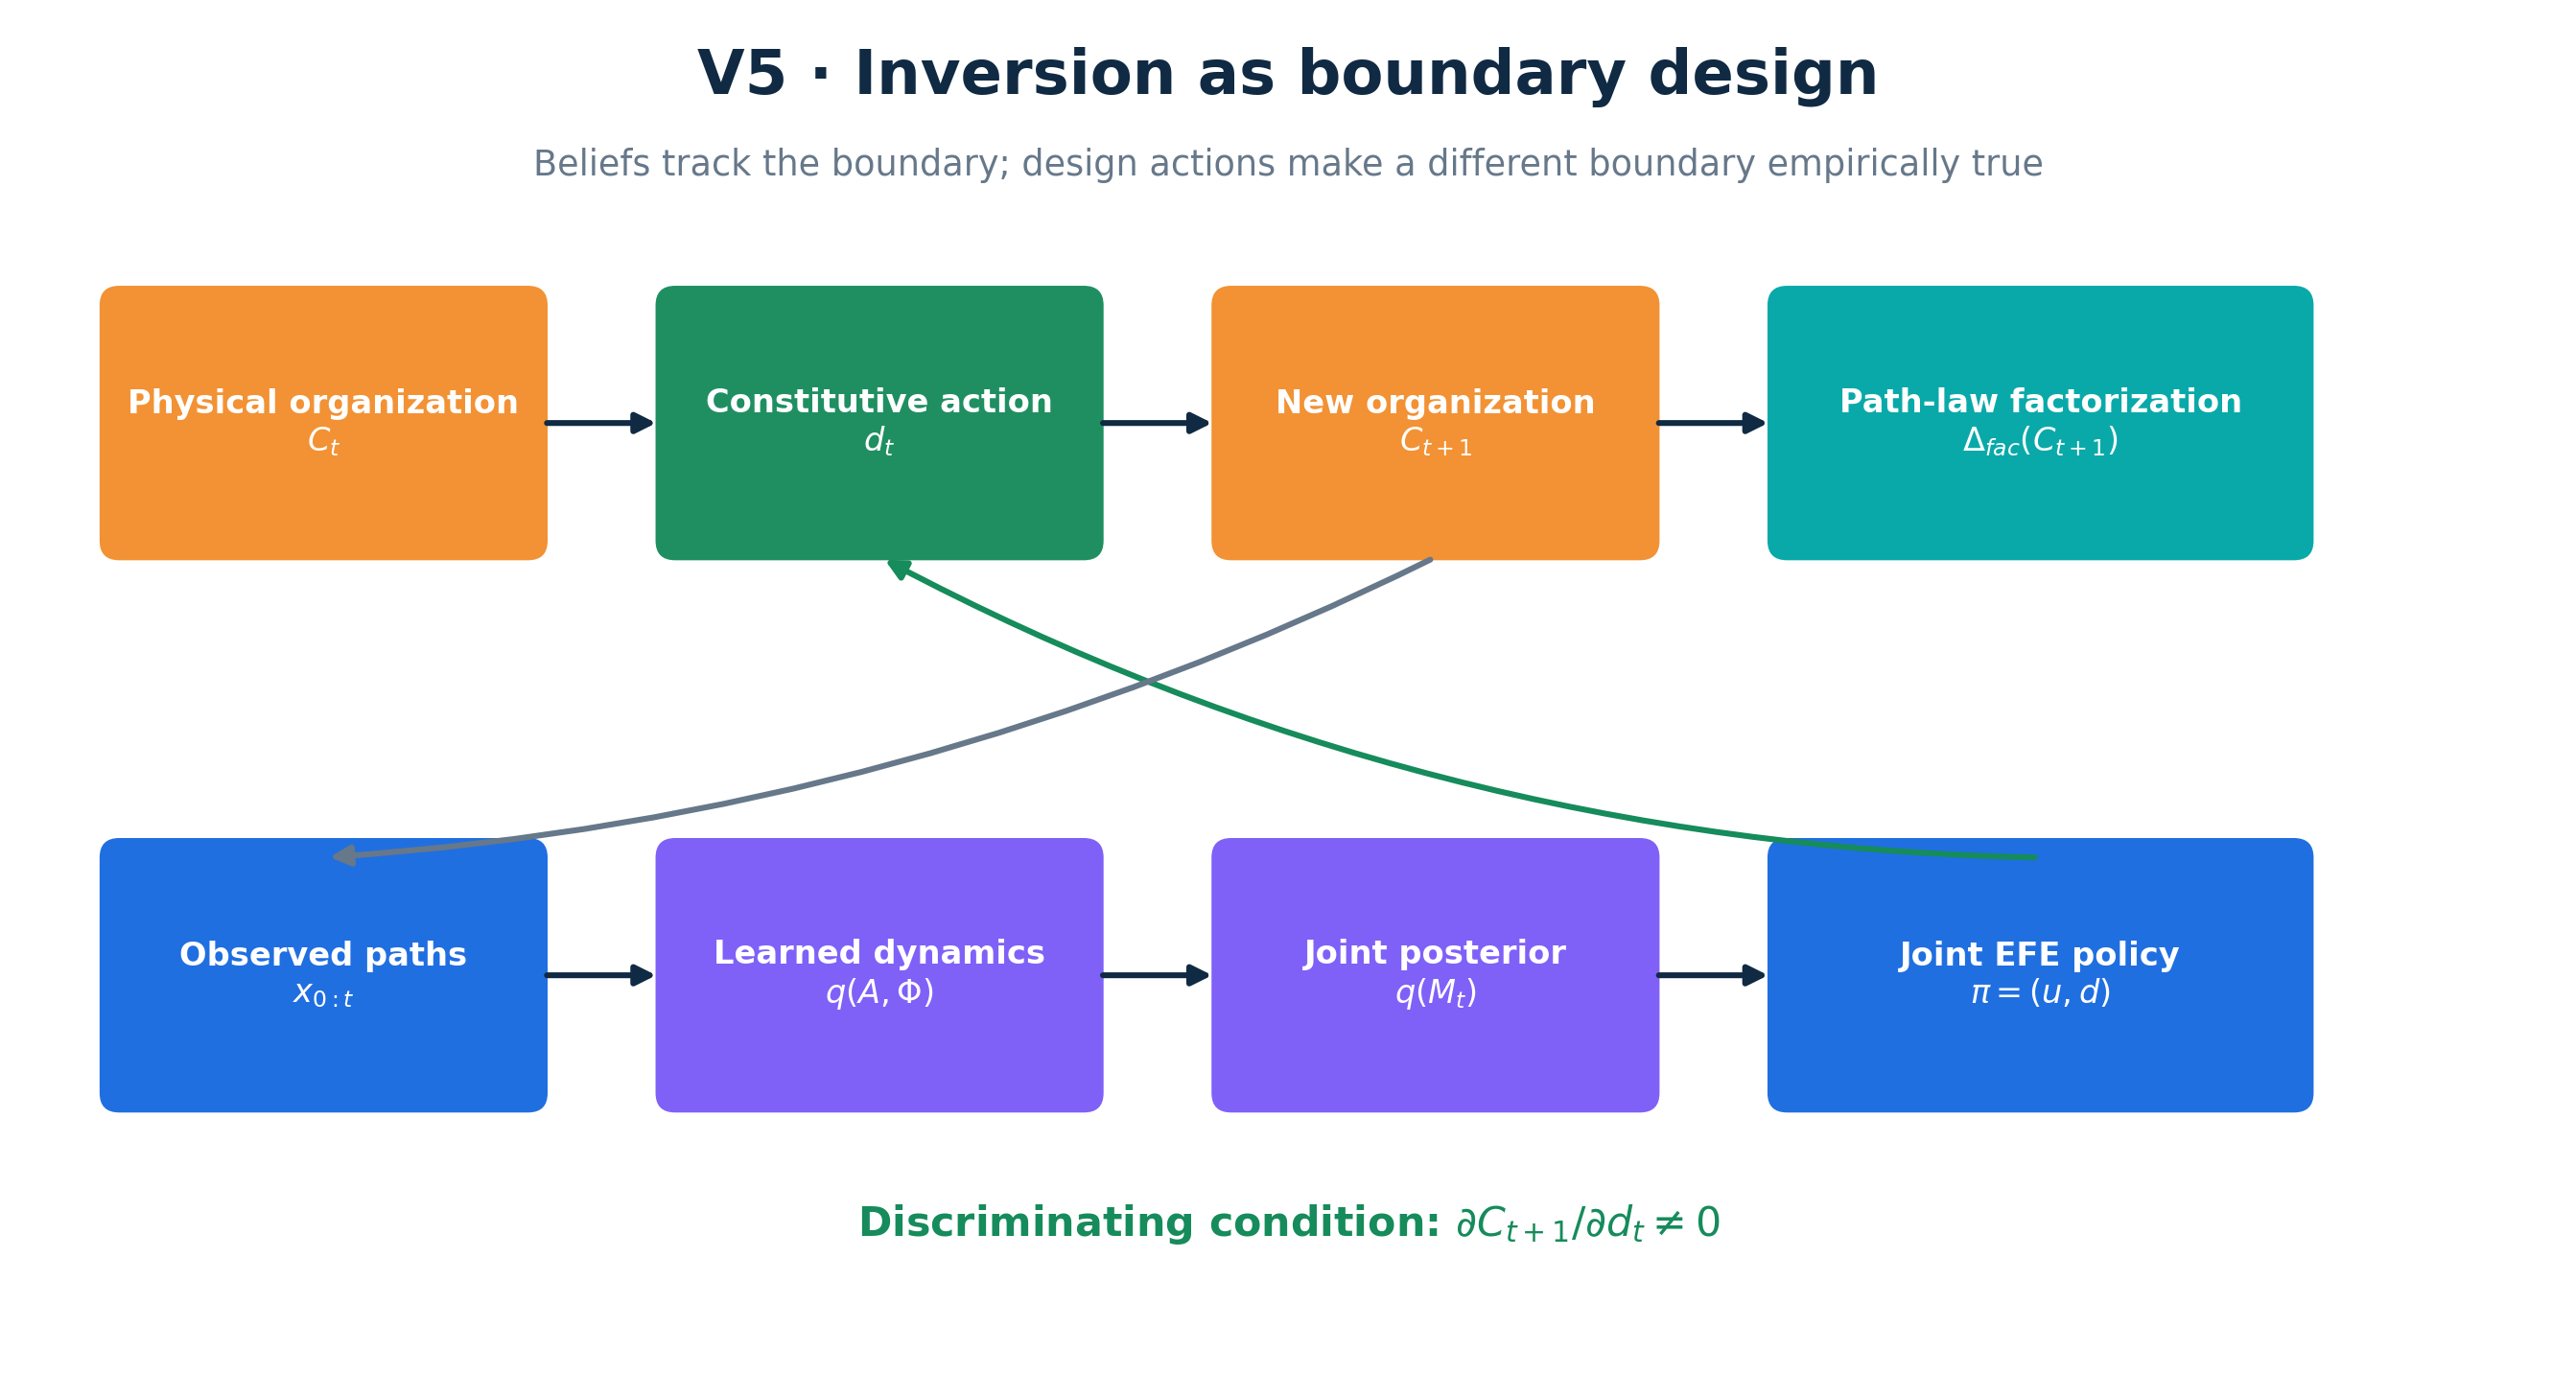
\includegraphics[width=\textwidth]{v5_architecture.png}
  \caption{V5 separates physical causal organization $\Corg_t$ from the
  posterior $q_t(M)$. The lower loop learns and evaluates; the upper loop is
  changed by constitutive design action.}
  \label{fig:architecture}
\end{figure}

\section{FEP, Active Inference, and Design}

\subsection{Variational free energy}

Let $o$ denote observations, $z$ hidden states, $p(o,z)$ a generative model,
and $q(z)$ a variational density. Variational free energy is
\begin{align}
  F[q;o]
  &= \E_{q(z)}[\ln q(z)-\ln p(o,z)] \\
  &= \KL\!\left[q(z)\,\|\,p(z\mid o)\right]-\ln p(o).
  \label{eq:vfe}
\end{align}
Because the KL divergence is nonnegative, $F\ge -\ln p(o)$. Minimizing $F$
with respect to $q$ makes the approximate posterior approach the Bayesian
posterior. This identity is a statement about inference; stronger claims
about organisms or artifacts require additional assumptions about dynamics,
ergodicity, and the partition of states \cite{friston2010,friston2019,
millidge2021,parr2022,buckley2017,clark2017}.

Under active inference, actions are included in policies $\pi$. A standard
expected-free-energy functional for future outcomes $o_\tau$ and states
$z_\tau$ can be written
\begin{align}
  G_\tau(\pi)
  &= \E_{q(o_\tau,z_\tau\mid\pi)}
     [\ln q(z_\tau\mid\pi)-\ln p(o_\tau,z_\tau)] \\
  &\approx
  \underbrace{\E_{q(o_\tau\mid\pi)}[-\ln p^*(o_\tau)]}_{\text{risk}}
  +\underbrace{\E_{q(z_\tau\mid\pi)}
    [\Hent(p(o_\tau\mid z_\tau))]}_{\text{ambiguity}}
  -\underbrace{\MI_q(z_\tau;o_\tau\mid\pi)}_{\text{epistemic value}},
  \label{eq:efe}
\end{align}
where $p^*(o)$ encodes preferred outcomes. Equation~\eqref{eq:efe} matters
because policy selection is not only reward maximization. Policies can be
valuable because they are expected to resolve uncertainty
\cite{parrfriston2017,dacosta2020,parr2022,friston2015efe,
friston2017process,pezzulo2015,tschantz2020}.

\subsection{Markov blankets and paths}

A blanket is sometimes presented as a static graphical separator. That is
insufficient here. The drone acts and learns through histories, and hidden
memory can preserve interior--exterior dependence even when
Equation~\eqref{eq:fixed-blanket} holds at a single time. Sakthivadivel's
path-space analysis treats the boundary as a factorization of regular
conditional laws \cite{sakthivadivel2026}:
\begin{equation}
 P(\mathrm dY_{[0,T]},\mathrm dX_{[0,T]}\mid B_{[0,T]})
 =P(\mathrm dY_{[0,T]}\mid B_{[0,T]})
  P(\mathrm dX_{[0,T]}\mid B_{[0,T]}).
 \label{eq:path-factor}
\end{equation}
When exact factorization fails, the residual dependence is the conditional
mutual information
\begin{equation}
 \MI(Y_{[0,T]};X_{[0,T]}\mid B_{[0,T]})
 =\E_{B}\KL\!\left[P_{Y,X\mid B}\,
 \middle\|\,P_{Y\mid B}P_{X\mid B}\right].
 \label{eq:path-cmi}
\end{equation}
For diffusions, Girsanov's theorem connects changes of path law to quadratic
control energy. This supplies the mathematical reason V5 measures direct
unscreened drift rather than only comparing role labels.

\subsection{From inference to design theory}

Existing work has already connected active inference to niche construction,
material engagement, cultural affordances, human--computer interaction, and
the design of intelligible artificial systems
\cite{bruineberg2018,constant2018,constant2021,veissiere2020,
albarracin2024,friston2024ecosystems,murraysmith2025}. These approaches show
how an agent changes its environment, selects observations, or externalizes
generative models. They are essential antecedents, but most begin with an
agent--environment partition that remains analytically fixed.

Multi-agent active-inference research has modeled generalized synchrony,
belief alignment, collective intelligence, and social niche construction
\cite{palacios2019,kaufmann2021,ramstead2020}. Those models motivate the
second experiment but do not by themselves settle its question. Synchrony or
shared prediction can arise between agents whose individual boundaries remain
fixed. Part~II instead makes the group partition a latent and controllable
variable and requires that a group-level intervention be irreducibly
bilateral.

Possati's difference is the level at which design operates. The primary
design variable is the partition itself: which states mediate inward and
outward influence, which dependencies are screened off, and which histories
become conditionally independent. This is not simply ``active inference
applied to design.'' It is a design-theoretic interpretation of individuation
in which an interface is an achieved causal-statistical organization.

Three operations from the book receive explicit computational counterparts:
\begin{itemize}
  \item \textbf{Precision crafting} becomes the selection, gating, routing,
  and calibration of sensor and actuator modules. Precision is not only an
  inference weight; it is changed by altering which physical module occupies
  a boundary port.
  \item \textbf{Curiosity sculpting} becomes the EFE-guided choice of
  structural perturbations. The drone selects which coupling to test or
  change because of its expected epistemic and pragmatic value.
  \item \textbf{Prediction embedding} becomes priors over complete role
  partitions together with learned transition and intervention likelihoods.
  Expectations are embedded in a material routing architecture, not held only
  as symbolic forecasts.
\end{itemize}

\section{Inversion as the Design of a Boundary}

\subsection{Detection, tracking, and constitution}

Let $M_t$ be a hypothesis about roles and let $\Corg_t$ be the actual causal
organization. Detection asks whether $q_t(M)$ identifies a fixed
$\Corg_t$. Tracking asks whether $q_t(M)$ follows exogenous changes in
$\Corg_t$. Constitution asks whether the artifact selects $d_t$ such that
\begin{equation}
 \Corg_{t+1}=\Tmap(\Corg_t,d_t,\omega_t),
 \label{eq:constitutive-transition}
\end{equation}
where $\omega_t$ collects exogenous disturbances, and such that the selected
action changes the causal relations that define the boundary.

This separation corrects the central limitation of V4. In that model, a
script exchanged thermal and optic-flow roles and probes returned noisy role
cues from a known likelihood. The agent could detect and track the script,
but the intervention did not create or remodel the boundary. V5 contains no
exogenous role exchange. Exogenous events can damage precision or open a
causal breach, but only a drone-selected routing or shielding action can
produce the repaired or transformed organization.

\begin{figure}[t]
 \centering
 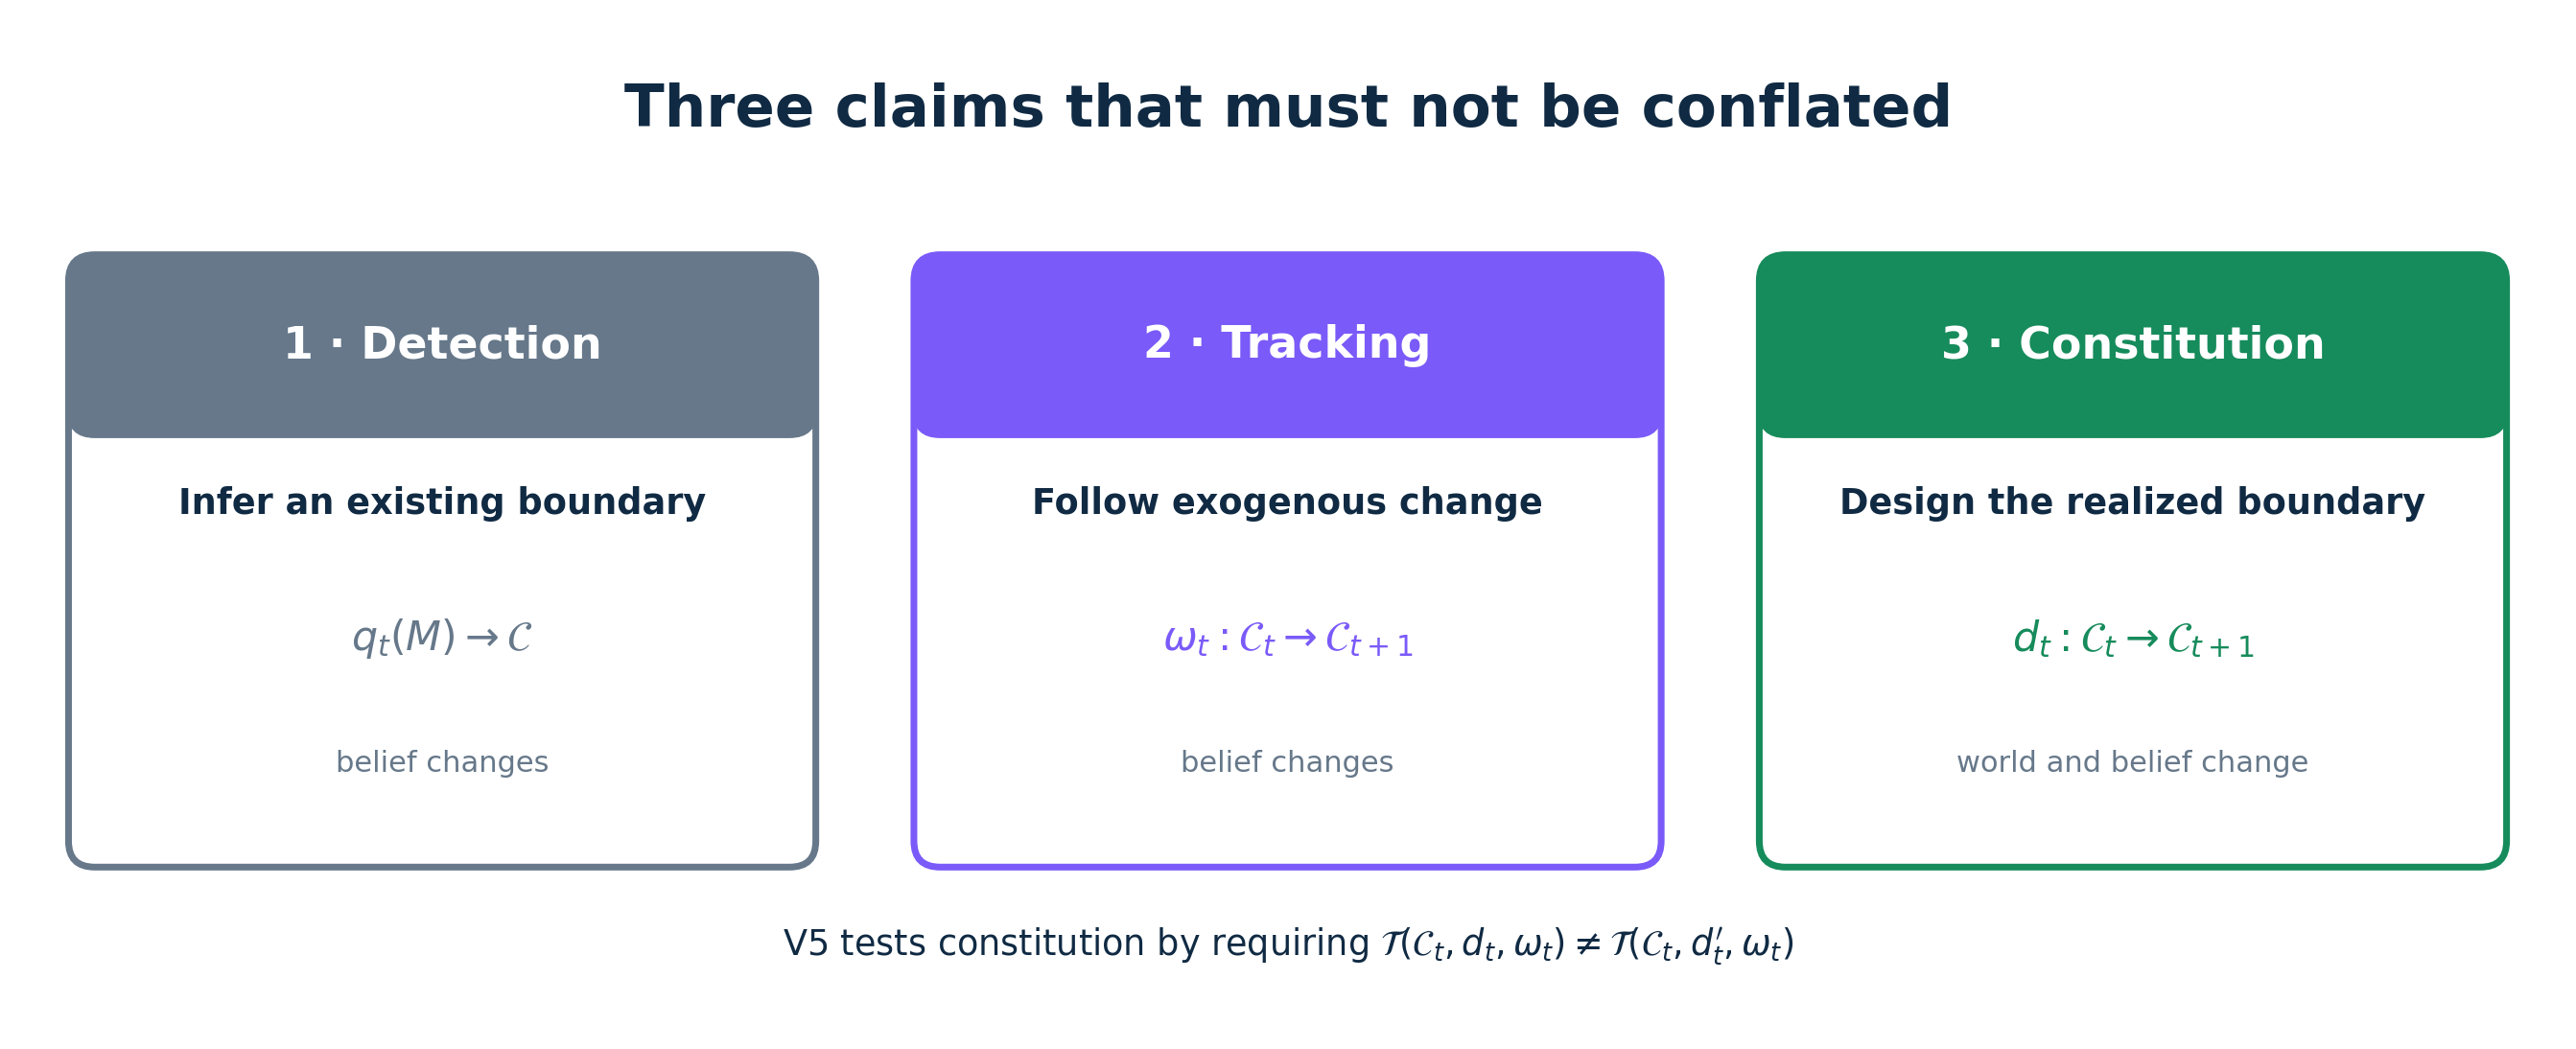
\includegraphics[width=0.96\textwidth]{inversion_levels.png}
 \caption{Three increasingly strong meanings of structural inversion.
 Detection estimates a fixed organization; tracking follows an organization
 changed from outside; constitution closes the loop by allowing the selected
 design action to alter the organization that generates future paths.}
 \label{fig:inversion-levels}
\end{figure}

\subsection{The narrow thesis tested here}

The model tests a bounded proposition:
\begin{quote}
Given a finite candidate state space, a finite repertoire of physically
effective interventions, and online evidence about dynamics and precision,
a joint EFE policy can select actions that improve path-law factorization and
viability more reliably than an otherwise identical diagnostic policy.
\end{quote}
This proposition is weaker than open-ended self-construction. It is also
stronger than structural classification, because the dependent variable is
the causal process itself.

\subsection{Why this is specifically Possati's inversion}

Beck and Ramstead invert a generative model in order to identify a
macroscopic organization: observed microscopic dynamics provide evidence for
which variables occupy blanket roles \cite{beckramstead2025}. Possati retains
that inferential movement but adds its practical reverse. Once a provisional
organization has been inferred, an artifact can act on the couplings that
support it. The output of model inversion becomes an input to design; design
then changes the data-generating organization and initiates another round of
inversion. The resulting loop is
\begin{equation}
 \text{paths}\longrightarrow q_t(M)\longrightarrow d_t
 \longrightarrow \Corg_{t+1}\longrightarrow\text{new paths}.
 \label{eq:possati-loop}
\end{equation}
This is the book's discriminating claim in computational form. The boundary
is neither merely given by the engineer nor merely discovered by the agent.
It is a revisable achievement whose causal support can be constructed,
maintained, or redirected.

The three design notions used throughout the paper are correspondences, not
decorative analogies. \emph{Precision crafting} is implemented by sensor and
actuator selection, gating, routing, and calibration. \emph{Curiosity
sculpting} is implemented by EFE-selected structural perturbations whose
epistemic value depends on the current partition posterior. \emph{Prediction
embedding} is implemented by priors over complete role assignments and by
learned likelihoods over dynamics and intervention outcomes. In Part~II these
operations are distributed across two bodies: precision is jointly routed,
curiosity must be agreed, and predictions are embedded in a pooled group
model.

\part{Individual Boundary Design}

\section{Complete Mathematical Model}

\subsection{State space and four-role partitions}

There are $n=8$ generic modules $V=\{1,\ldots,8\}$. A role map is
\begin{equation}
 r:V\rightarrow\{\Irole,\Srole,\Arole,\Erole\}.
 \label{eq:role-map}
\end{equation}
The experiment fixes two modules per role. The hypothesis space is therefore
\begin{equation}
 \Mset=\left\{r:\sum_{j=1}^{8}\mathbf 1[r(j)=k]=2,
 \quad k\in\{\Irole,\Srole,\Arole,\Erole\}\right\},
 \qquad |\Mset|=\frac{8!}{(2!)^4}=2520.
 \label{eq:partition-space}
\end{equation}
The agent maintains a joint posterior $q_t(M)$ over $\Mset$. Marginal role
probabilities are derived, not independently normalized:
\begin{equation}
 q_t(r_j=k)=\sum_{M\in\Mset}q_t(M)\mathbf 1[M(j)=k].
 \label{eq:marginals}
\end{equation}
Consequently, every posterior sample is a complete valid partition. The two
nodes within each role are exchangeable; evaluation is therefore insensitive
to their order.

\subsection{Physical causal organization}

The causal state is
\begin{equation}
 \Corg_t=(r_t,W_t,L_t,\rho_t),
 \label{eq:causal-state}
\end{equation}
where $r_t$ is the physical port assignment, $W_t\in\R^{8\times8}$ is a
directed drift matrix, $L_t$ is a set of unscreened links, and
$\rho_t\in[0,1]^8$ is module precision. Columns of $W$ are causes and rows
are effects. A clean template contains the directed cycle
\begin{equation}
 \Erole\longrightarrow\Srole\longrightarrow\Irole
 \longrightarrow\Arole\longrightarrow\Erole,
 \label{eq:role-cycle}
\end{equation}
plus stable within-role recurrence. All other cross-role entries are zero.
The template is scaled so its spectral radius is at most $0.82$.

The module dynamics are linear Gaussian:
\begin{equation}
 x_{t+1}=W(\Corg_t)x_t+b_A(r_t)u_t+b_E(r_t)w_t+\varepsilon_t,
 \qquad \varepsilon_t\sim\mathcal N(0,\Sigma_t).
 \label{eq:dynamics}
\end{equation}
Here $u_t$ is drone control, $w_t$ is an autocorrelated wind disturbance,
$b_A$ injects control into modules currently occupying active ports, and
$b_E$ injects wind into modules occupying external ports.

\subsection{A computable path-space gap}

Let $W_{IE}$ and $W_{EI}$ be the direct drift blocks between current internal
and external states. In a linear diffusion with isotropic innovation scale
$\sigma$, removing those blocks changes the conditional path law. The
quadratic Girsanov/Foellmer energy yields the benchmark measure
\begin{equation}
 \Gap(\Corg_t)=\frac{1}{2\sigma^2}
 \left(\|W_{IE}\|_F^2+\|W_{EI}\|_F^2\right).
 \label{eq:gap}
\end{equation}
It is zero for the simulated clean blanket and positive for a direct
interior--exterior drift channel. In this controlled linear-Gaussian setting,
Equation~\eqref{eq:gap} is a local relative-entropy-rate surrogate for the
path conditional mutual information in Equation~\eqref{eq:path-cmi}. It is
not claimed to be a universal metric for nonlinear physical systems.

\subsection{Constitutive interventions}

The design action is $d_t\in\mathcal D=\{d^0,d^{\mathrm{shield}}_{ij},
d^{\mathrm{swap}}_{ij}\}$. The actions have persistent effects:
\begin{align}
 d^{\mathrm{shield}}_{ij}:&\quad
 (W_{ij},W_{ji})\mapsto(0,0)
 \quad\text{when }(i,j)\in L_t, \\
 d^{\mathrm{swap}}_{ij}:&\quad
 (r_t(i),r_t(j))\mapsto(r_t(j),r_t(i)).
 \label{eq:design-actions}
\end{align}
Swapping changes which physical modules occupy the relevant causal ports
while preserving exactly two nodes per role. Shielding can make
Equation~\eqref{eq:path-factor} true by eliminating a bypass channel.

The diagnostic-only control evaluates the same nominal actions and pays the
same decision costs, but its transition is
\begin{equation}
 \Tmap_{\mathrm{diag}}(\Corg_t,d_t,\omega_t)
 =\Tmap_{\mathrm{diag}}(\Corg_t,d^0,\omega_t).
 \label{eq:diagnostic-null}
\end{equation}
This is the crucial negative control.

\subsection{Learned dynamics and structural posterior}

From a rolling window of transitions, the agent estimates $W$ by ridge
regression. With design matrix $Z=[X,U,\mathbf 1]$ and successor matrix $X^+$,
\begin{equation}
 \widehat\Theta_t=(Z^\top Z+\lambda I)^{-1}Z^\top X^+,
 \qquad \widehat W_t=(\widehat\Theta_{1:8})^\top.
 \label{eq:ridge}
\end{equation}
For every $M\in\Mset$, let $T_M$ denote its directed role template. The
structural log score is
\begin{equation}
 \ell_t(M)=-\tau\|\,|\widehat W_t|-T_M\|_F^2
 +\eta_A s_A(M;\widehat\Theta_t)
 +\eta_E s_E(M;\widehat\Sigma_t),
 \label{eq:structural-score}
\end{equation}
where $s_A$ measures alignment between learned control response and active
roles, and $s_E$ measures alignment between learned innovation variance and
external roles. Thus semantic orientation comes from learned response and
noise statistics, not a supplied table of role cues. The posterior is
\begin{equation}
 q_t(M)=\frac{\exp\ell_t(M)}{\sum_{M'\in\Mset}\exp\ell_t(M')}.
 \label{eq:partition-posterior}
\end{equation}
A small hazard mixture prevents premature certainty when the organization
changes.

\subsection{Learned intervention model}

For each intervention family $k\in\{\mathrm{shield},\mathrm{swap}\}$, let
$\theta_k$ be the probability that an attempted action produces an observable
causal change. V5 uses
\begin{equation}
 \theta_k\sim\mathrm{Beta}(a_k,b_k),\qquad
 (a_k,b_k)\leftarrow(a_k+c_t,b_k+1-c_t),
 \label{eq:beta-intervention}
\end{equation}
where $c_t=1$ exactly when the pre/post causal matrices differ. The predictive
success probability and variance are
\begin{equation}
 \widehat p_k=\frac{a_k}{a_k+b_k},\qquad
 \mathrm{Var}(\theta_k)=\frac{a_kb_k}{(a_k+b_k)^2(a_k+b_k+1)}.
 \label{eq:beta-moments}
\end{equation}
The prior is $\mathrm{Beta}(1,1)$. This model is intentionally modest: it
learns family-level causal efficacy rather than receiving a known
role-conditioned probe likelihood.

\subsection{Precision and viability}

Let
\begin{equation}
 \bar\rho_S(t)=\frac{1}{2}\sum_{j:r_t(j)=\Srole}\rho_j(t),\qquad
 \bar\rho_A(t)=\frac{1}{2}\sum_{j:r_t(j)=\Arole}\rho_j(t).
 \label{eq:precision}
\end{equation}
The cross-track state $y_t$ evolves as
\begin{equation}
 y_{t+1}=0.91y_t+\delta\left(\widetilde w_t
 +1.22\bar\rho_A(t)u_t\right)+\xi_t,
 \quad
 \widetilde w_t\sim\mathcal N\!\left(w_t,
 \frac{0.20^2}{\bar\rho_S(t)^2}\right).
 \label{eq:viability-dynamics}
\end{equation}
Poor sensory routing therefore increases estimation noise; poor active routing
attenuates control. A collision occurs at $|y_t|>2.35$.

\subsection{Joint expected-free-energy policy}

A policy is the pair $\pi=(u,d)$. V5 scores all admissible pairs together:
\begin{align}
 G_t(u,d)
 &=R_t(u)+\alpha\,\mathcal A_t(u)
 +c(d) \\
 &\quad-\widehat p_{k(d)}
 \left[\beta_s V^{\mathrm{struct}}_t(d)
 +\beta_p V^{\mathrm{precision}}_t(d)\right]
 -\beta_I\,\mathrm{IG}_t(d).
 \label{eq:implemented-efe}
\end{align}
$R_t$ is predicted cross-track and control risk; $\mathcal A_t$ is predictive
ambiguity from transition residuals; $c(d)$ is intervention cost;
$V^{\mathrm{struct}}$ is the expected removal of an $I$--$E$ coupling under
the role posterior; $V^{\mathrm{precision}}$ is the expected benefit of
routing a precise module into a boundary port; and $\mathrm{IG}$ combines
local role entropy with intervention-model uncertainty. Policies are sampled
from
\begin{equation}
 q(\pi)\propto\exp[-G_t(\pi)/\gamma].
 \label{eq:policy-softmax}
\end{equation}
Equation~\eqref{eq:implemented-efe} is ``genuine EFE'' in the operational
sense that pragmatic risk, ambiguity, and expected information gain all alter
policy probability. It remains a finite-horizon approximation, not an exact
solution of a continuous-time variational control problem.

\section{Experimental Design}

\subsection{Three discriminating tasks}

\textbf{Construction.} Each mission starts with three direct $I$--$E$ links.
The agent constructs a boundary only by selecting the corresponding shielding
actions. Successful construction requires a final gap below 10\% of its
initial value and no collision.

\textbf{Stabilization.} The mission begins with a clean boundary. At a
seed-random time between steps 27 and 38, one direct $I$--$E$ channel opens.
Roles do not change. Successful stabilization requires a final gap below
$0.25$ and no collision.

\textbf{Transformation.} The mission begins with a clean boundary. At a
seed-random time between steps 31 and 42, one current boundary module loses
precision and one external module becomes highly precise. This event does not
change their roles. The drone must select a physical port swap. Successful
transformation requires the realized routing to match the new
precision-optimal partition and no collision. Both the old and new partitions
can have zero factorization gap, so the predicted effect is on boundary
precision and viability, not on $\Gap$.

\subsection{Conditions}

\begin{table}[t]
\centering
\small
\begin{tabularx}{\textwidth}{>{\bfseries}lX}
\toprule
Condition & Definition \\
\midrule
Constitutive & Joint EFE control and physically effective shield/swap actions. \\
Diagnostic only & Same nominal choices, but design actions cannot change $\Corg_t$. \\
Factorized & Control is selected first; design is selected separately from structural value. \\
Random design & A random structural action is paired with EFE control. \\
Passive & No structural action. \\
Oracle & Ground-truth breach or routing mismatch selects the design action. \\
\bottomrule
\end{tabularx}
\caption{Experimental conditions. The primary contrast is constitutive versus diagnostic only.}
\label{tab:conditions}
\end{table}

\subsection{Frozen protocol and outcomes}

The benchmark uses \NSeeds{} held-out paired seeds for each of six conditions
and three tasks, giving \NTotal{} missions. Exogenous random streams are paired
by seed and task. The primary outcomes are task success and final architecture
score
\begin{equation}
 Q_{\mathrm{arch}}=exp[-\Gap(\Corg_T)/8]
 \min\{\bar\rho_S(T),\bar\rho_A(T)\}.
 \label{eq:architecture-score}
\end{equation}
Secondary outcomes are viability, collision, mean and final gap, role
accuracy, blanket-set accuracy, exact final partition recovery, number of
causal changes, and recovery delay. Viability is a bounded function of mean
cross-track error, collision, and precision deficit.

A descriptive mediation analysis tests the proposed causal chain. With
$X=1$ for the constitutive condition, $M=Q_{\mathrm{arch}}$, and $Y$ equal to
viability, task-adjusted ordinary least squares estimates
\begin{equation}
 M=a_0+aX+\Gamma T+\epsilon_M,\qquad
 Y=b_0+c'X+bM+\Lambda T+\epsilon_Y.
 \label{eq:mediation}
\end{equation}
The indirect association $ab$ is bootstrapped by paired seed. This analysis is
supportive, not a substitute for the randomized primary contrast.

\section{Results}

\subsection{Primary constitutive test}

Figure~\ref{fig:benchmark} reports the frozen benchmark. The constitutive
agent succeeded in \ConstructFull\% of construction trials versus
\ConstructDiag\% for diagnostic only; \StabilizeFull\% versus
\StabilizeDiag\% in stabilization; and \TransformFull\% versus
\TransformDiag\% in transformation. The paired final-gap difference was
\ConstructGapDelta{} in construction and \StabilizeGapDelta{} in
stabilization. In transformation the final-gap contrast was zero by design,
while the paired viability difference was \TransformViabilityDelta{}.

\begin{figure}[t]
 \centering
 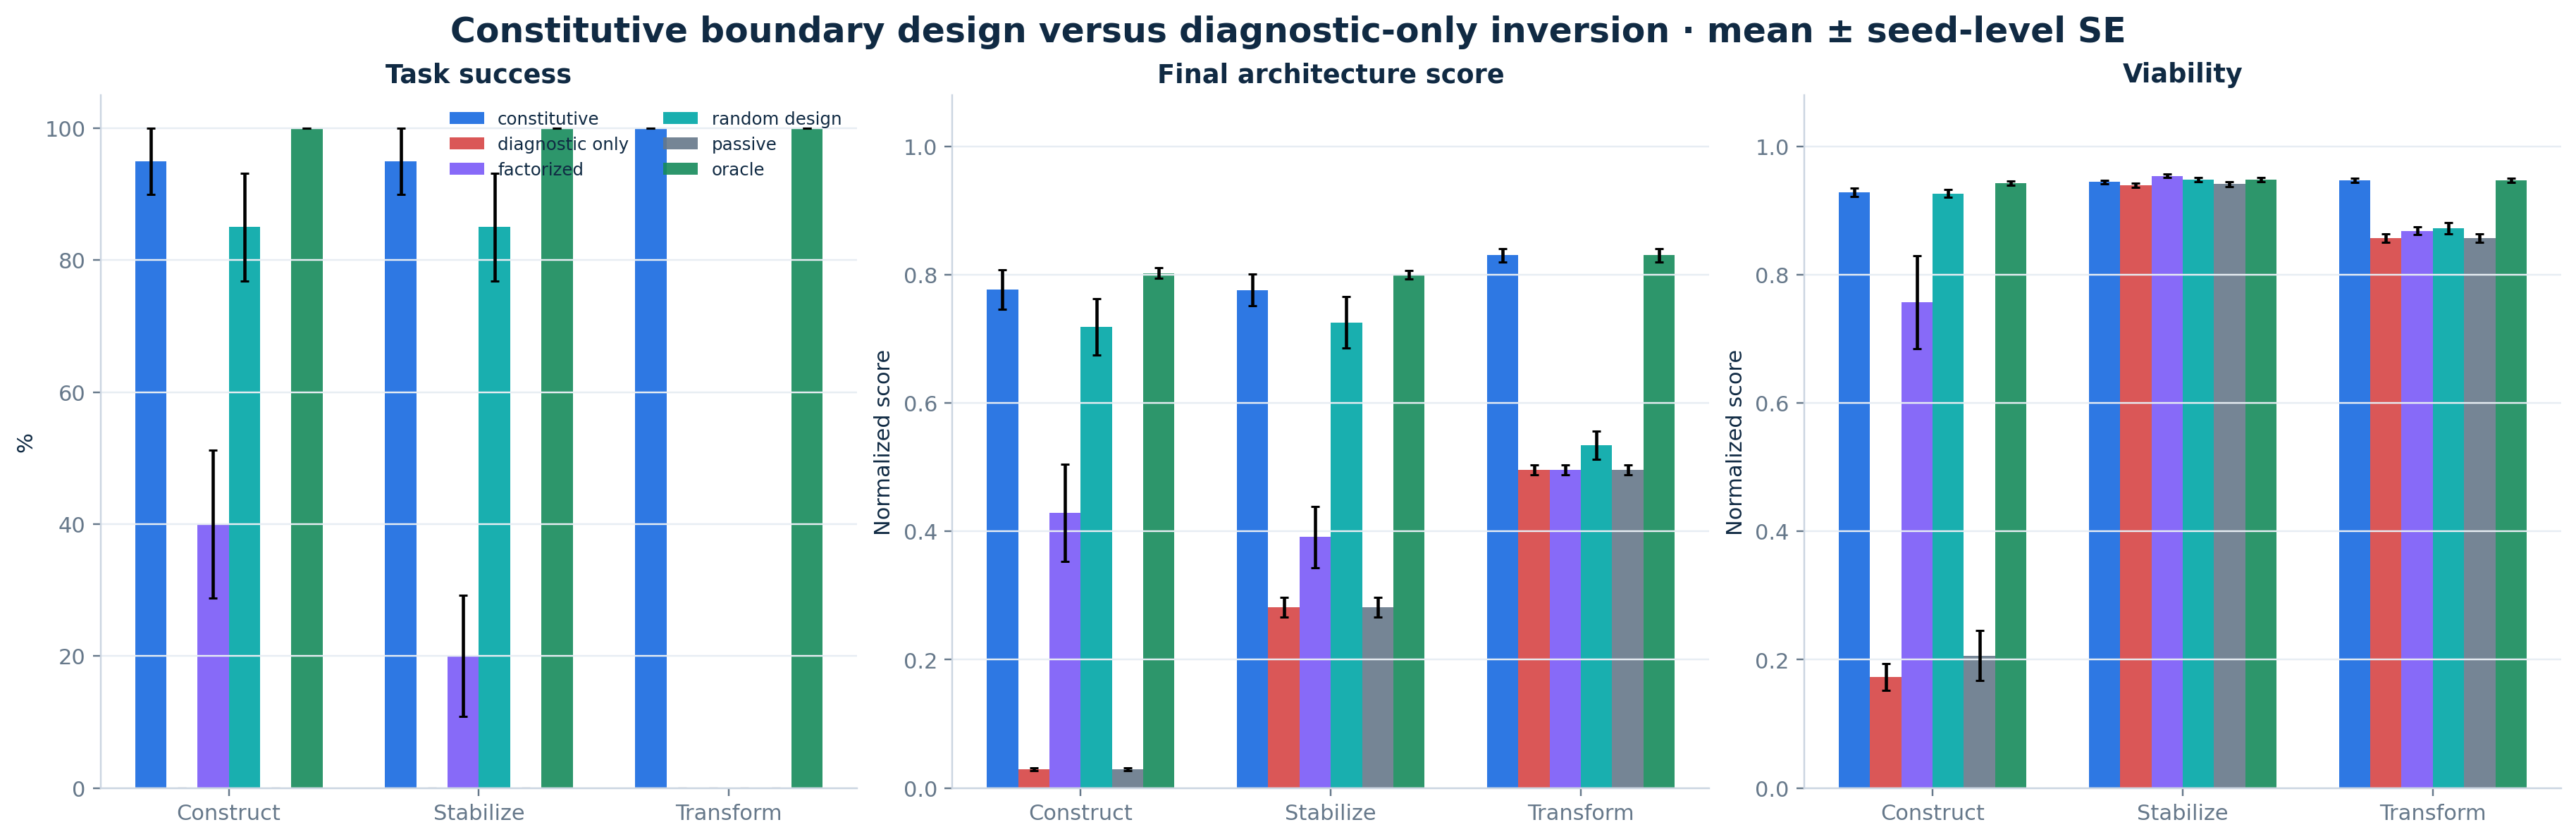
\includegraphics[width=\textwidth]{v5_benchmark.png}
 \caption{Task success, architecture score, and viability for the six
 conditions. Error bars are seed-level standard errors.}
 \label{fig:benchmark}
\end{figure}

The primary comparison therefore answers the V4 objection directly. The
diagnostic agent can update its model and can select nominal interventions,
but it cannot make the desired conditional independencies true. The
constitutive agent changes $W_t$ or $r_t$ and thereby changes the sampled path
law.

\subsection{Construct, stabilize, transform}

Figure~\ref{fig:triad} shows representative successful missions. Construction
requires three discrete causal changes and ends at zero gap. Stabilization
shows a seed-random breach followed by a selected repair. Transformation
contains no forced role switch: the precision event changes which routing is
useful, and a single swap performed by the drone changes the actual role map.

\begin{figure}[p]
 \centering
 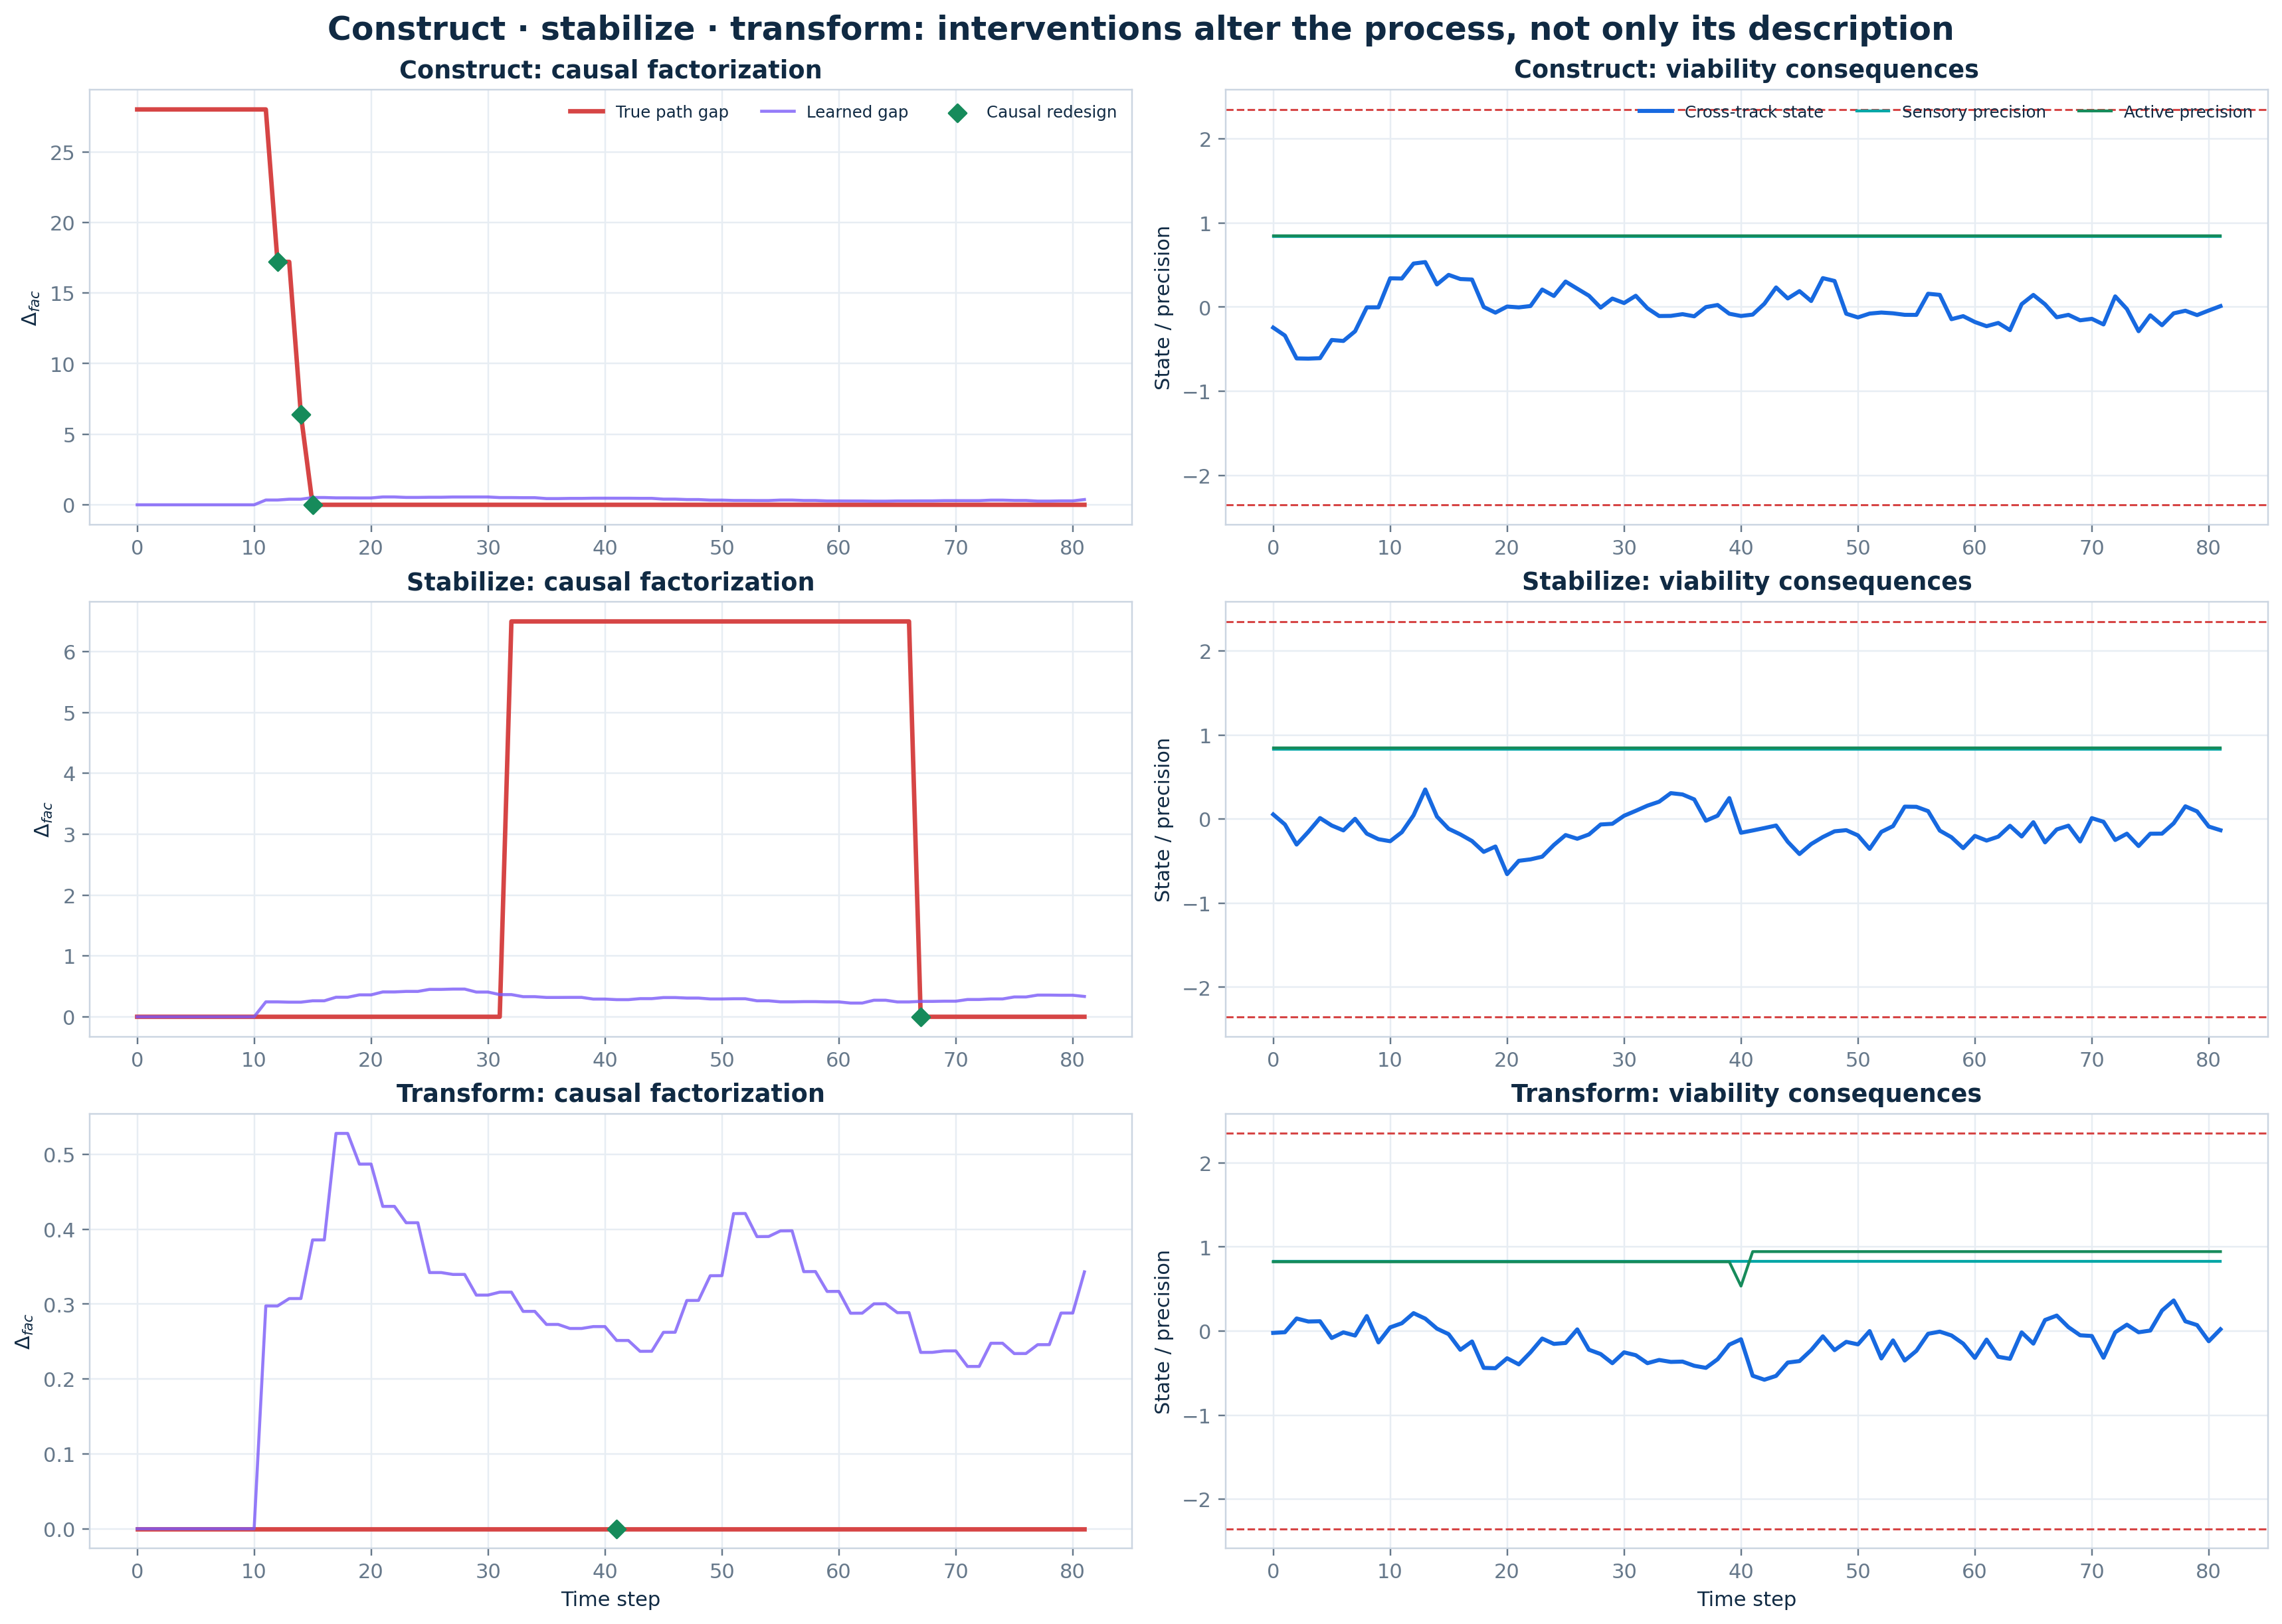
\includegraphics[width=\textwidth]{construct_stabilize_transform.png}
 \caption{Representative missions for the three design verbs. Green diamonds
 mark actions that changed the causal matrix.}
 \label{fig:triad}
\end{figure}

\subsection{Complete role inference}

V5 does not use four independent classifiers. The posterior ranges over
complete partitions and produces marginals only by Equation~\eqref{eq:marginals}.
Figure~\ref{fig:roles} displays the four posterior fields in a transformation
mission. Internal states are no longer an anchored target omitted from
discovery; they are inferred jointly with sensory, active, and external roles.

\begin{figure}[p]
 \centering
 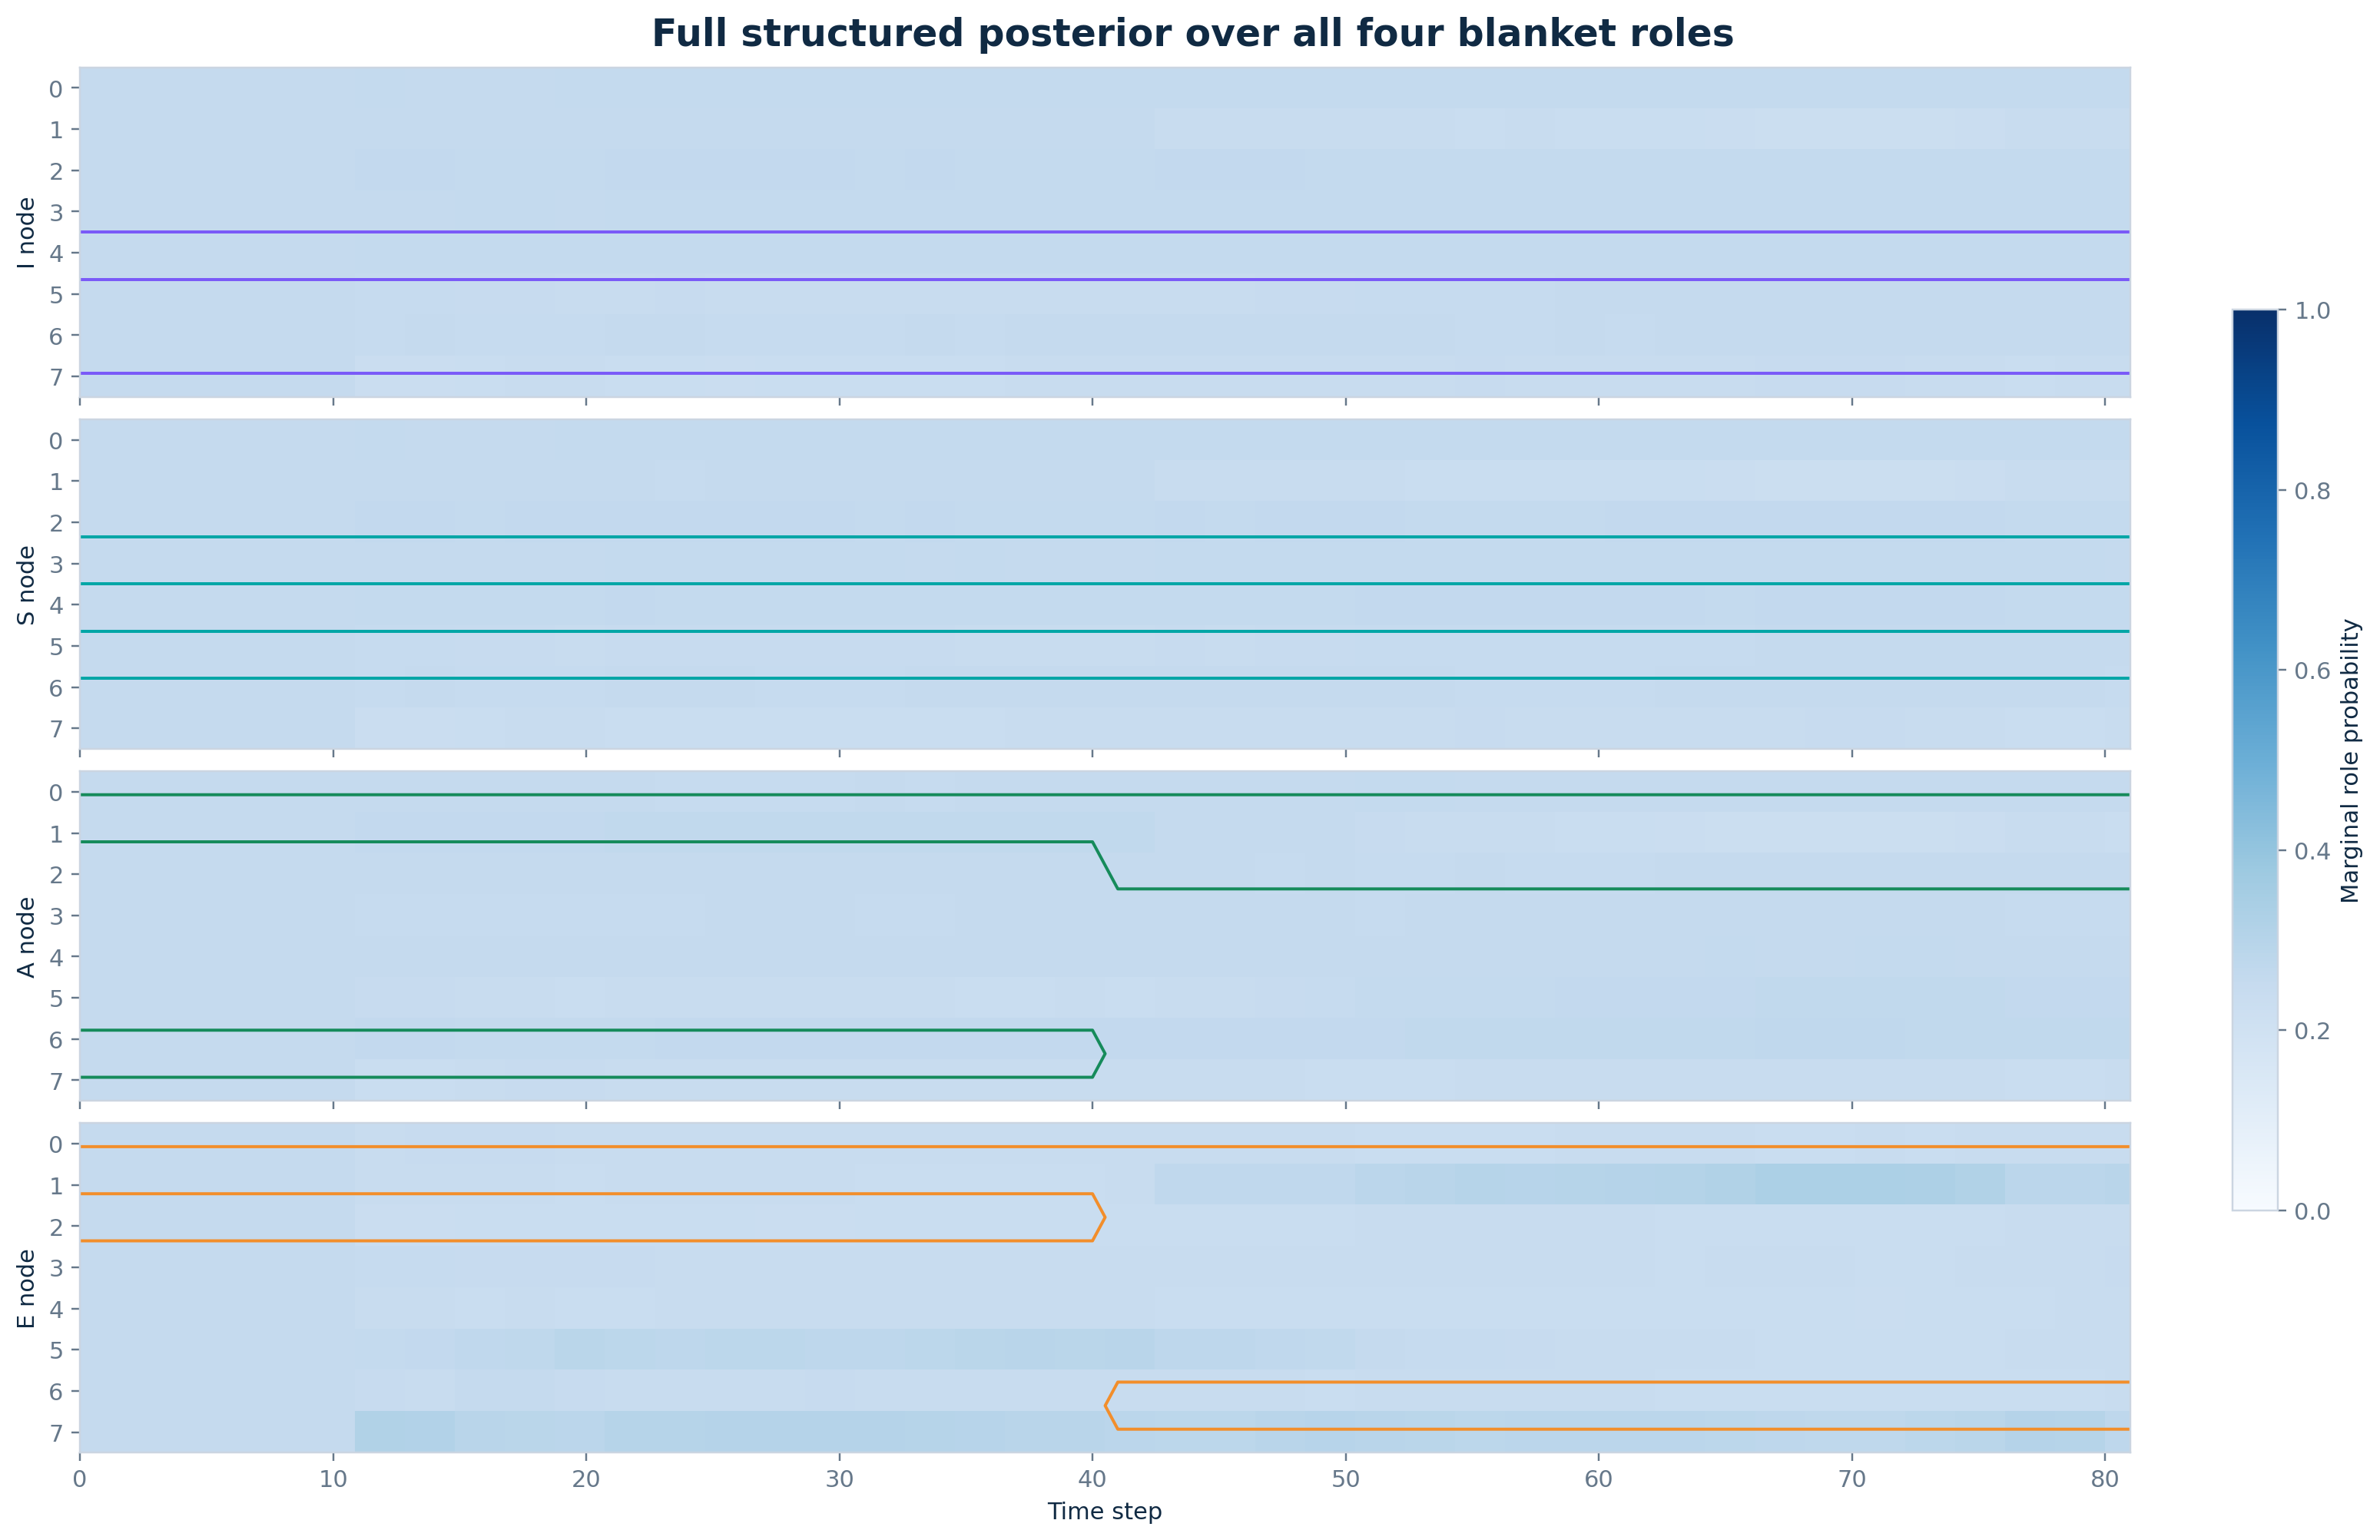
\includegraphics[width=\textwidth]{four_role_posterior.png}
 \caption{Posterior role probabilities for all eight modules and all four
 roles. Contours indicate the physical role assignment.}
 \label{fig:roles}
\end{figure}

\subsection{Architecture and viability}

Across the constitutive and diagnostic conditions, the task-adjusted indirect
association through architecture score was \ArchitectureIndirect{}
(paired-seed bootstrap 95\% interval
[\ArchitectureIndirectLow{}, \ArchitectureIndirectHigh{}]). This is
consistent with the proposed chain
\begin{equation}
 d_t\longrightarrow\Corg_{t+1}\longrightarrow
 \text{factorization/precision}\longrightarrow\text{viability}.
 \label{eq:causal-chain}
\end{equation}
The result should be interpreted cautiously: the mediator is partly defined
from simulator-level variables and the simple regression does not prove a
general mechanistic law.

\subsection{Ablations and process diagnostics}

The ablation matrix in Figure~\ref{fig:individual-ablation} shows why success
alone is insufficient. Random design can sometimes close one of a small
number of breaches, but it does not solve targeted transformation; the
factorized controller separates motor regulation from design and therefore
misses interactions between structural and ordinary action. The oracle
defines an attainable ceiling. The constitutive controller approaches that
ceiling without access to the true role map.

\begin{figure}[p]
 \centering
 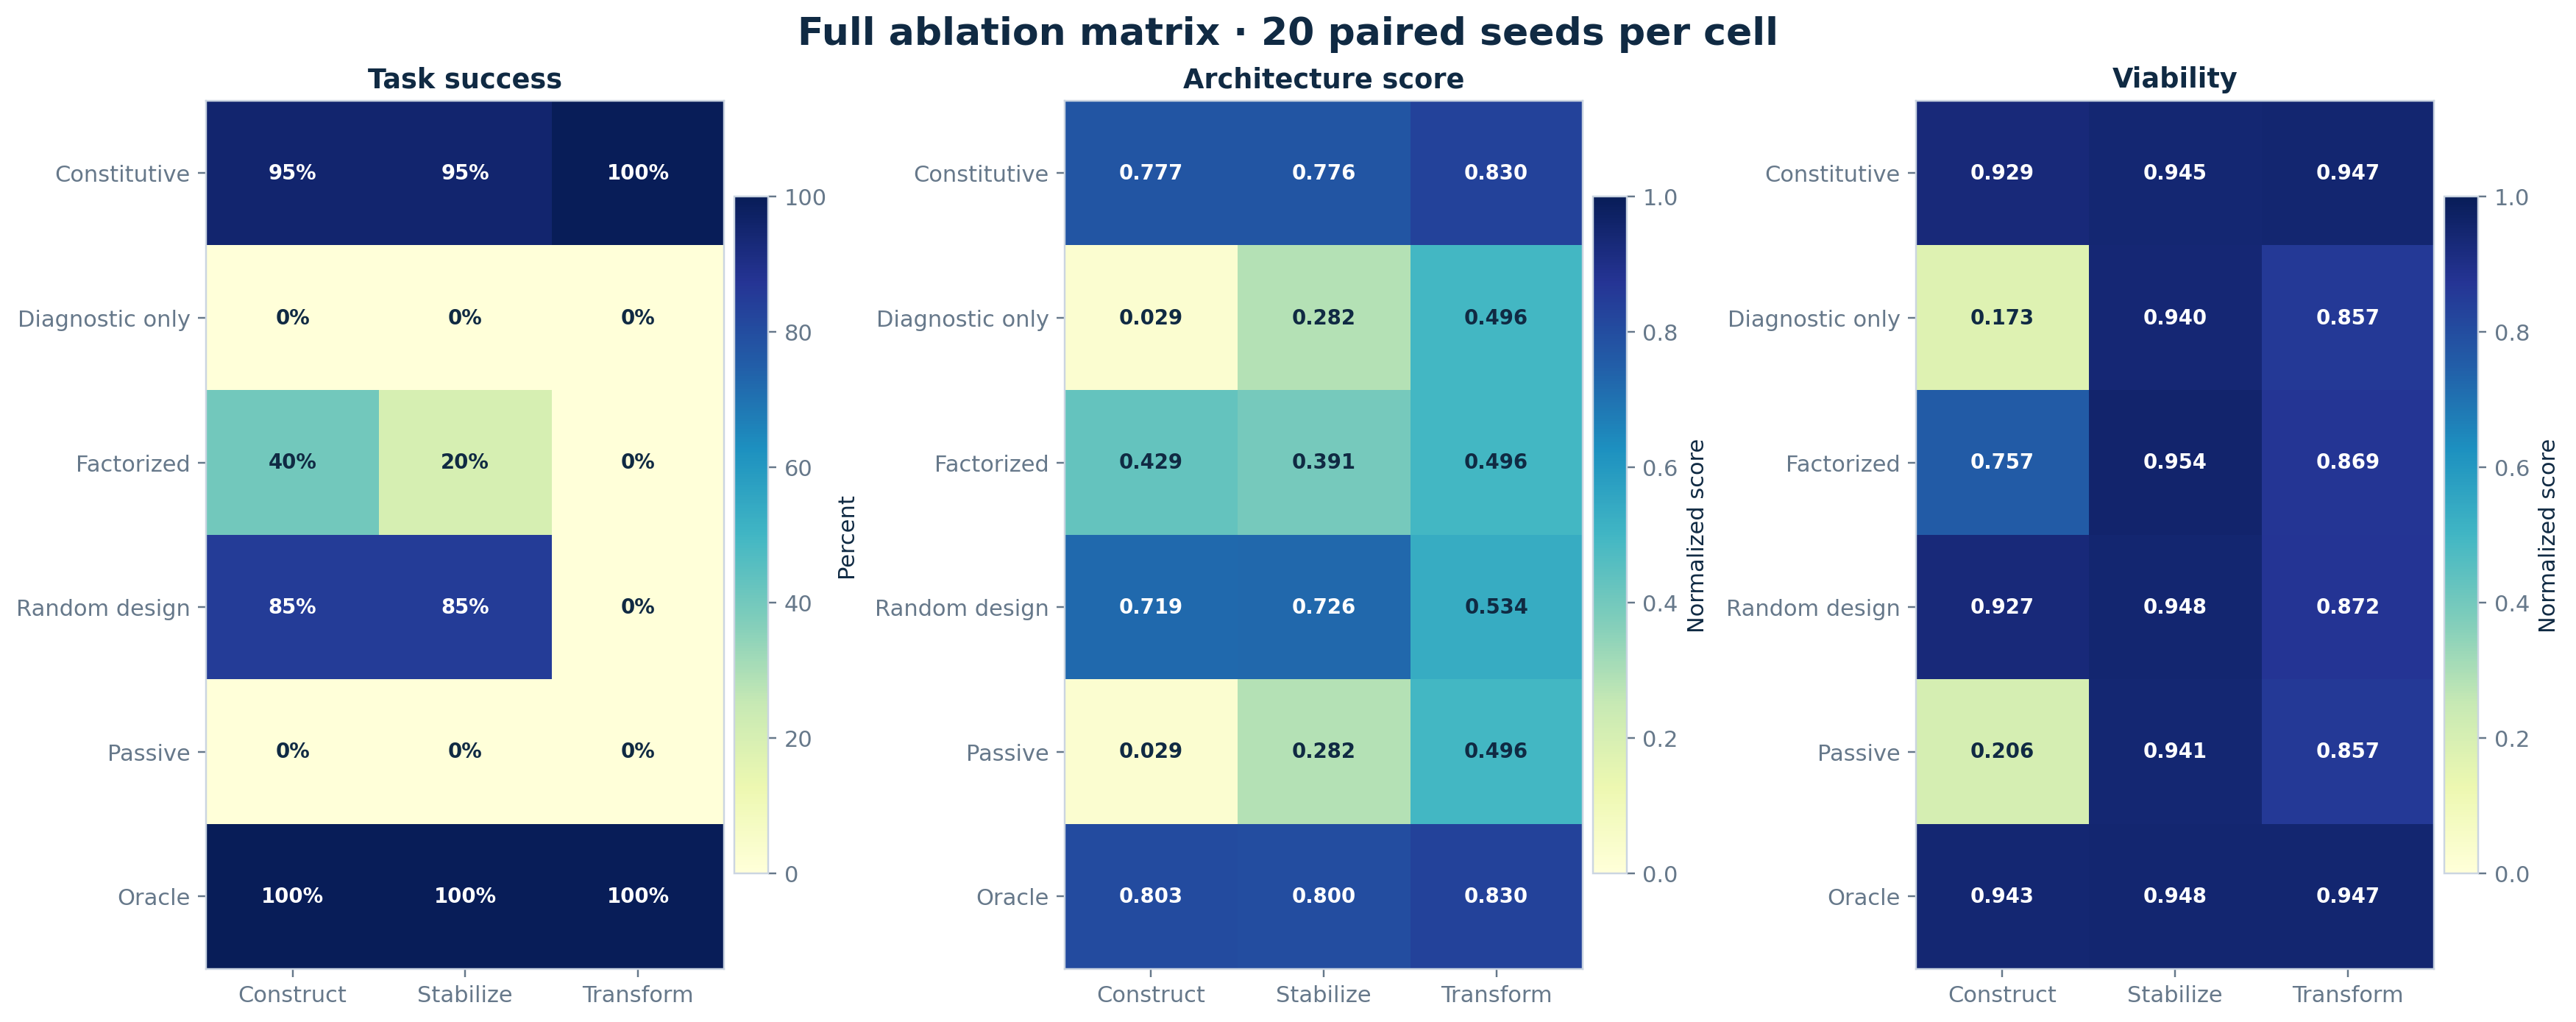
\includegraphics[width=0.98\textwidth]{ablation_matrix.png}
 \caption{Part~I ablation matrix. Each cell is a mean over the same 20 paired
 seeds. The architecture score distinguishes a merely surviving trajectory
 from one supported by the intended factorization and boundary precision.}
 \label{fig:individual-ablation}
\end{figure}

Figure~\ref{fig:efe-components} makes the controller auditable. Risk favors
stabilizing motor commands, ambiguity penalizes noisy predictions, epistemic
value favors actions expected to distinguish role hypotheses, and structural
value favors actions expected to close a bypass or improve routed precision.
Because all terms are evaluated on the pair $(u,d)$, the value of a design
operation depends on the control action with which it will be executed.

\begin{figure}[p]
 \centering
 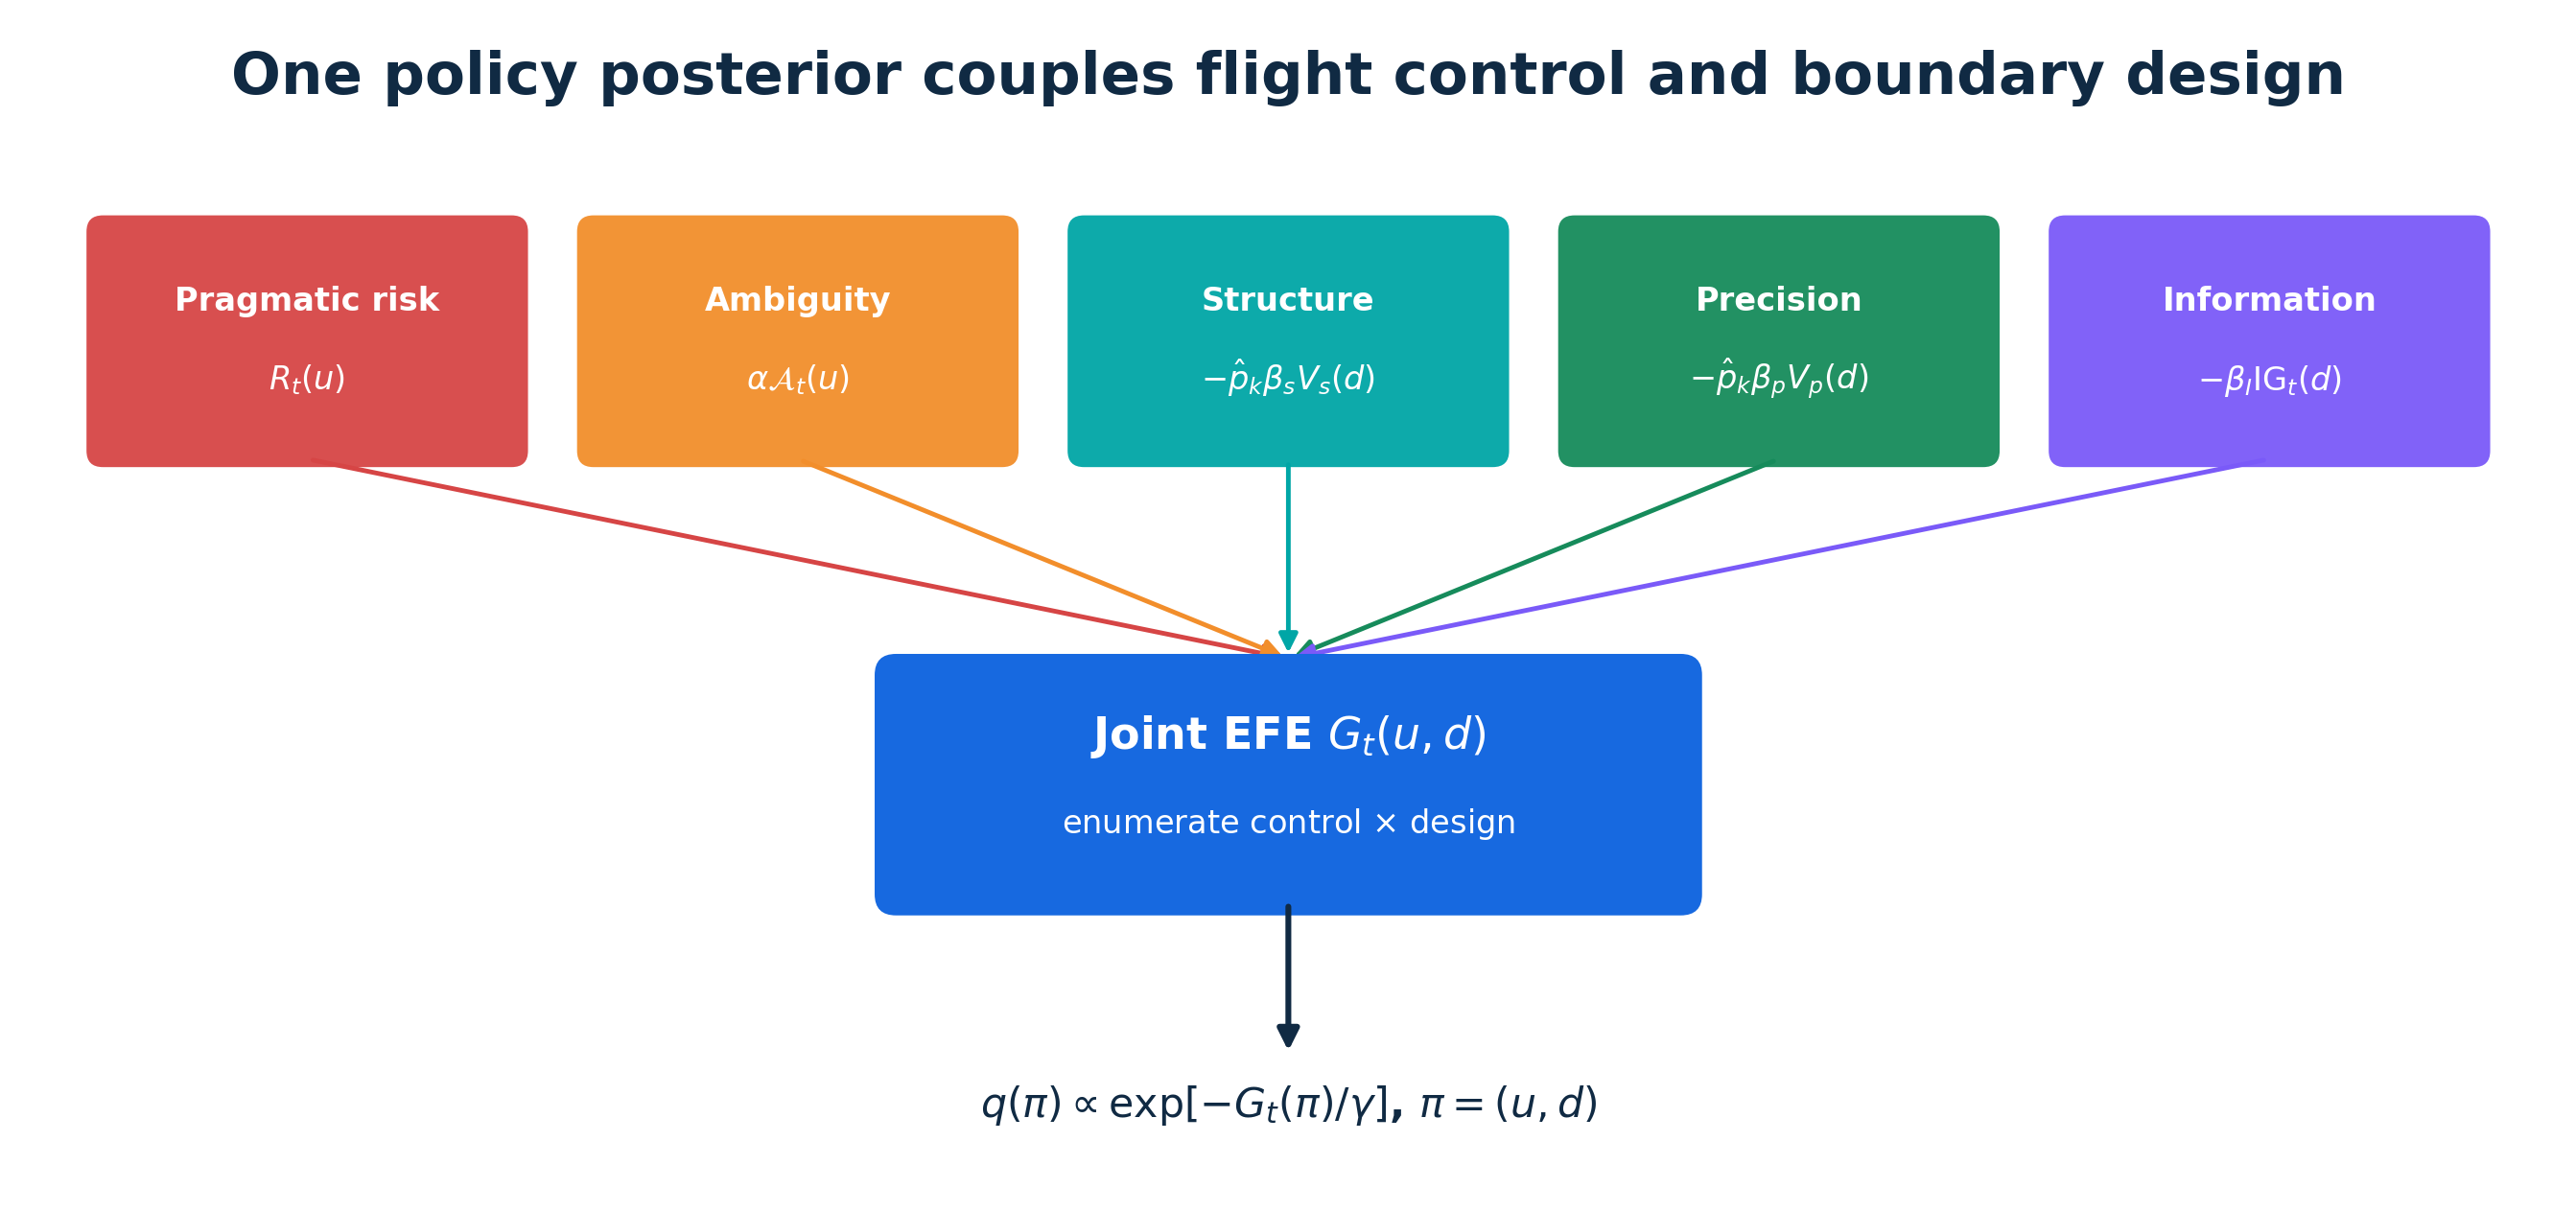
\includegraphics[width=0.95\textwidth]{joint_efe_decomposition.png}
 \caption{Implemented EFE decomposition and policy ranking in representative
 decisions. The chart reports the actual terms used by the controller rather
 than a post-hoc verbal classification.}
 \label{fig:efe-components}
\end{figure}

The paired trajectories in Figure~\ref{fig:paired-chain} hold the exogenous
random stream fixed and vary only whether the selected structural action is
allowed to modify $\Corg_t$. This comparison localizes the intervention:
posterior updating occurs in both conditions, but only the constitutive arm
changes the path-space gap and routed precision. Figure~\ref{fig:diagnostics}
adds posterior entropy, action timing, and intervention-model learning.

\begin{figure}[p]
 \centering
 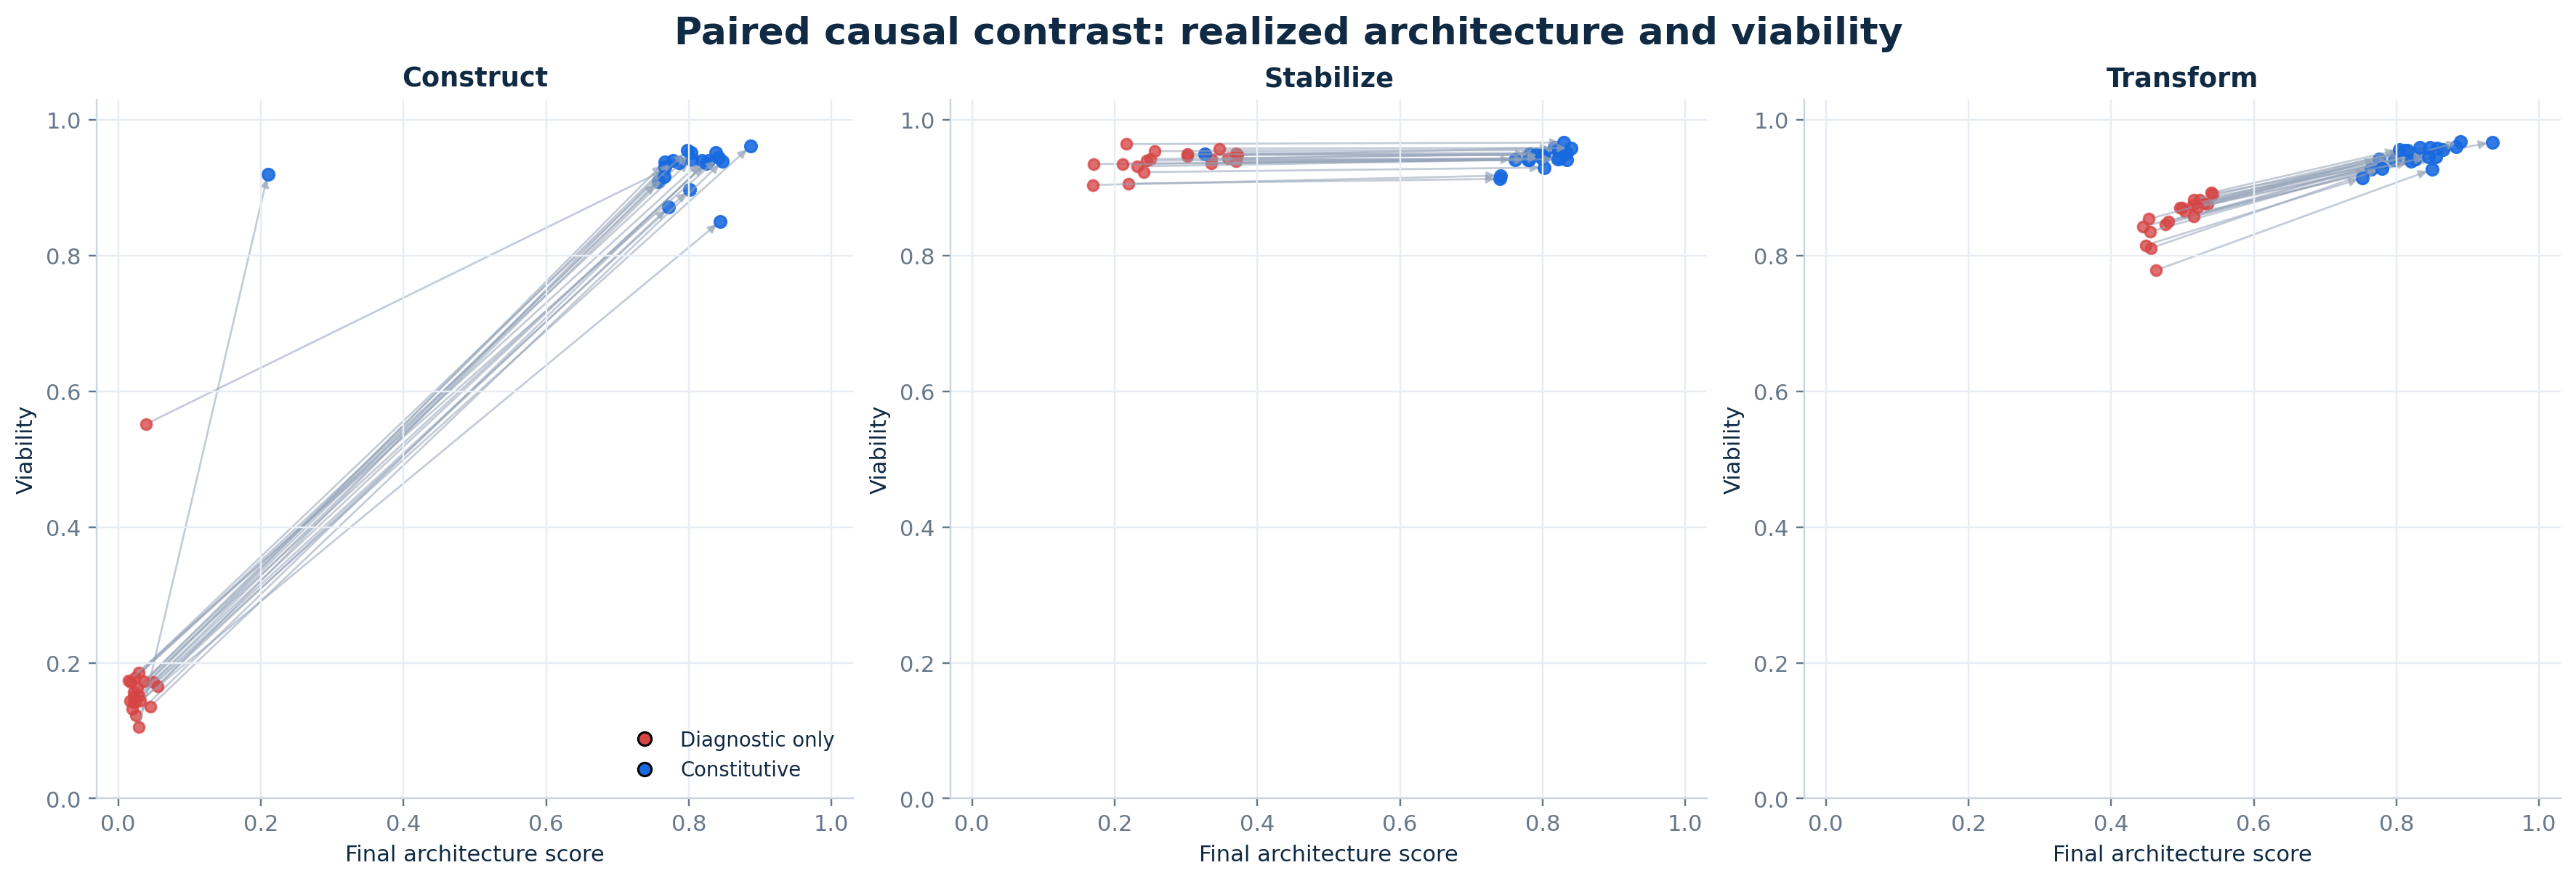
\includegraphics[width=\textwidth]{paired_causal_chain.png}
 \caption{Paired causal-chain diagnostics. Within each seed, the constitutive
 and diagnostic runs share disturbances; the difference is the physical
 efficacy of design action.}
 \label{fig:paired-chain}
\end{figure}

\begin{figure}[p]
 \centering
 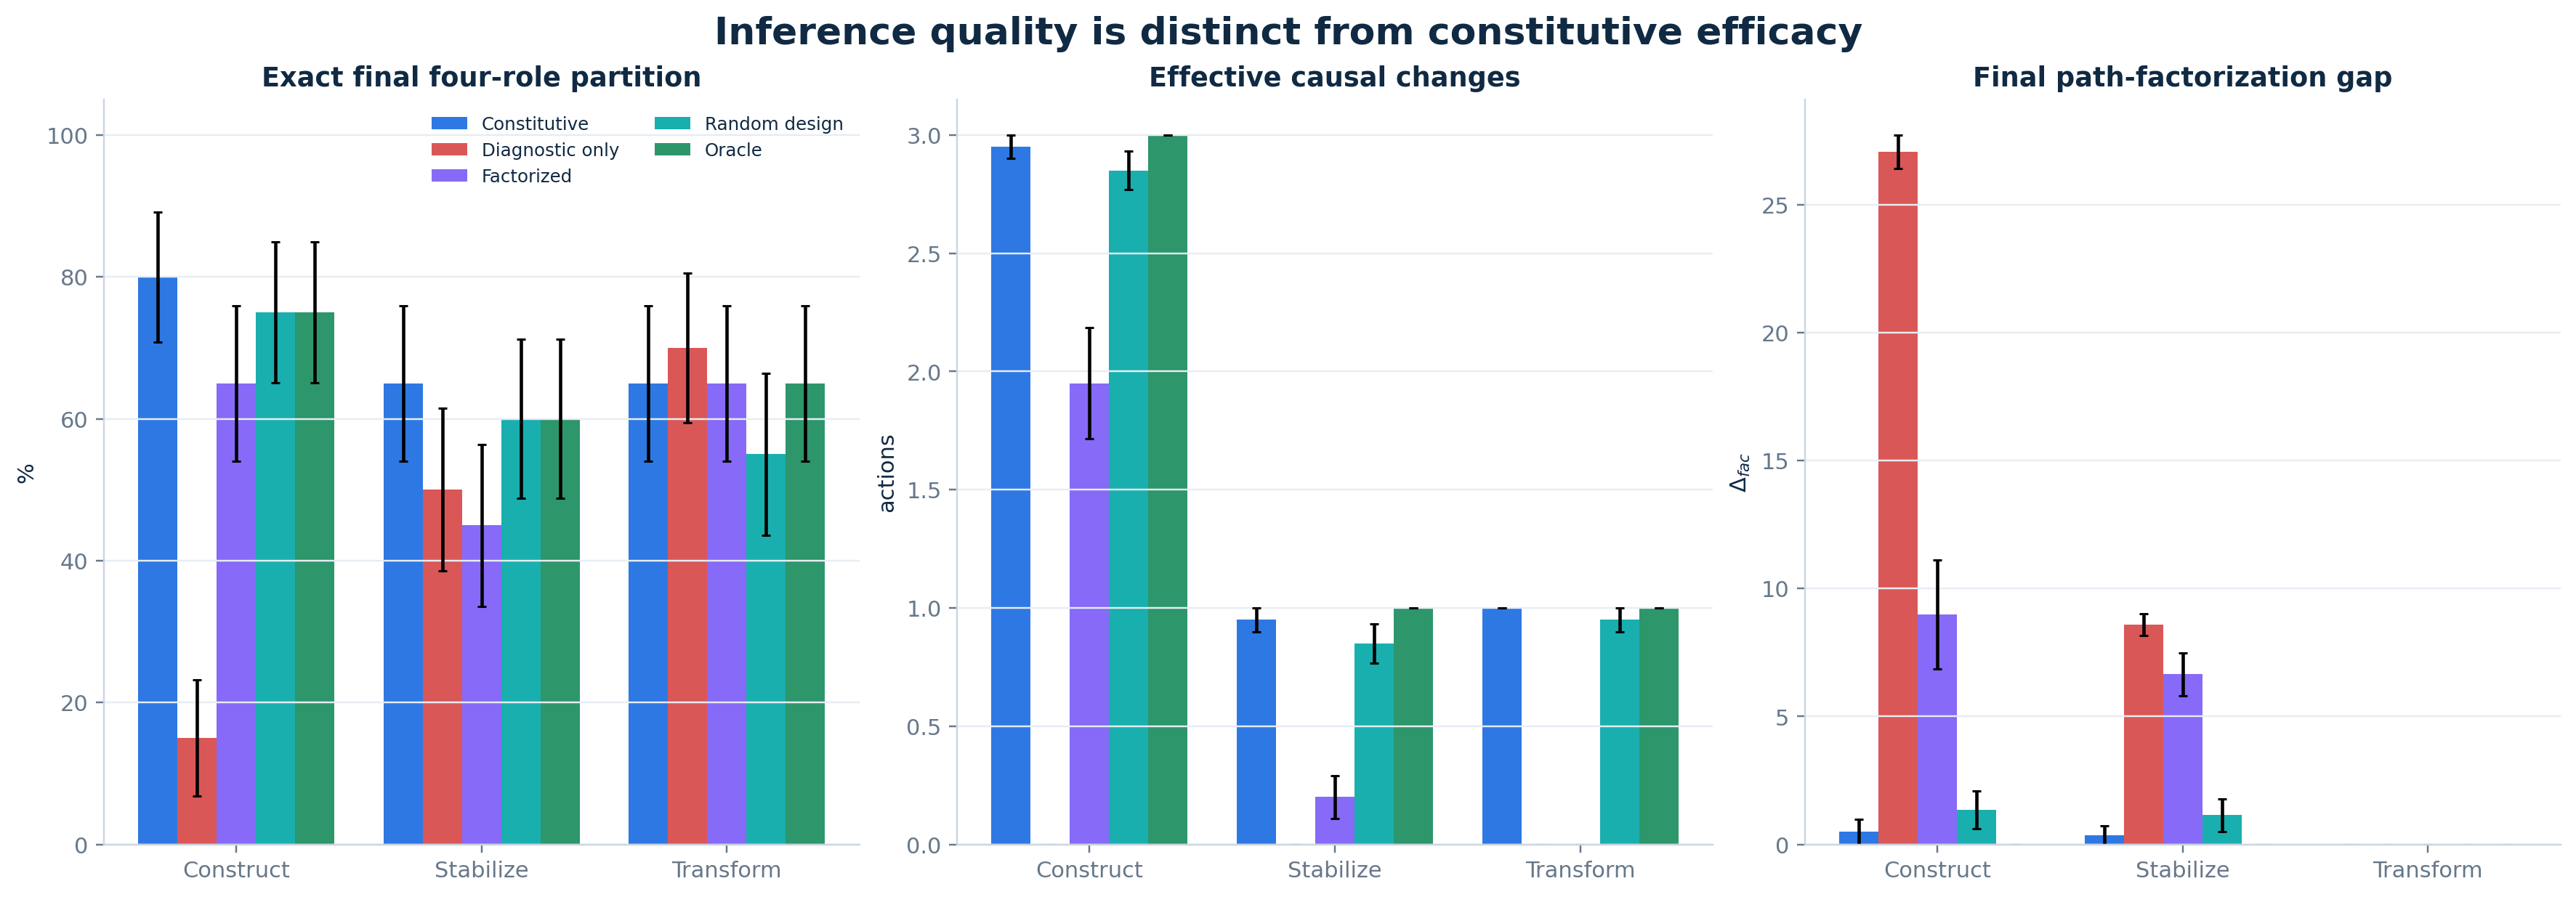
\includegraphics[width=\textwidth]{inference_action_diagnostics.png}
 \caption{Inference and action diagnostics. Structural uncertainty need not
 vanish before useful action: policy value integrates posterior uncertainty,
 learned efficacy, and predicted architectural benefit.}
 \label{fig:diagnostics}
\end{figure}

\begin{table}[p]
\centering
\scriptsize
\setlength{\tabcolsep}{3.7pt}
\begin{tabular}{llrrrrrr}
\toprule
Condition & Task & Success & Viability & $Q_{arch}$ & Final $\Delta_{fac}$ & Role acc. & Exact \\
\midrule
Constitutive & Construct & 95.0\% & 0.929 & 0.777 & 0.498 & 65.2\% & 80.0\% \\
Constitutive & Stabilize & 95.0\% & 0.945 & 0.776 & 0.359 & 78.6\% & 65.0\% \\
Constitutive & Transform & 100.0\% & 0.947 & 0.830 & 0.000 & 71.6\% & 65.0\% \\
\addlinespace[2pt]
Diagnostic only & Construct & 0.0\% & 0.173 & 0.029 & 27.068 & 49.4\% & 15.0\% \\
Diagnostic only & Stabilize & 0.0\% & 0.940 & 0.282 & 8.589 & 76.3\% & 50.0\% \\
Diagnostic only & Transform & 0.0\% & 0.857 & 0.496 & 0.000 & 78.6\% & 70.0\% \\
\addlinespace[2pt]
Factorized & Construct & 40.0\% & 0.757 & 0.429 & 8.979 & 61.1\% & 65.0\% \\
Factorized & Stabilize & 20.0\% & 0.954 & 0.391 & 6.652 & 72.2\% & 45.0\% \\
Factorized & Transform & 0.0\% & 0.869 & 0.496 & 0.000 & 76.3\% & 65.0\% \\
\addlinespace[2pt]
Random design & Construct & 85.0\% & 0.927 & 0.719 & 1.349 & 66.2\% & 75.0\% \\
Random design & Stabilize & 85.0\% & 0.948 & 0.726 & 1.142 & 74.8\% & 60.0\% \\
Random design & Transform & 0.0\% & 0.872 & 0.534 & 0.000 & 72.3\% & 55.0\% \\
\addlinespace[2pt]
Passive & Construct & 0.0\% & 0.206 & 0.029 & 27.068 & 49.1\% & 25.0\% \\
Passive & Stabilize & 0.0\% & 0.941 & 0.282 & 8.589 & 74.3\% & 55.0\% \\
Passive & Transform & 0.0\% & 0.857 & 0.496 & 0.000 & 78.6\% & 70.0\% \\
\addlinespace[2pt]
Oracle & Construct & 100.0\% & 0.943 & 0.803 & 0.000 & 72.8\% & 75.0\% \\
Oracle & Stabilize & 100.0\% & 0.948 & 0.800 & 0.000 & 76.6\% & 60.0\% \\
Oracle & Transform & 100.0\% & 0.947 & 0.830 & 0.000 & 71.6\% & 65.0\% \\
\bottomrule
\end{tabular}
\caption{Complete frozen benchmark. Values are means over 20 paired seeds.}
\label{tab:full-results}
\end{table}


\FloatBarrier
\part{Collective Boundary Design}

\section{From Coordination to Operational Individuation}

Part~II raises the scale of the question. Two drones may coordinate while
remaining two independently bounded agents: they can exchange positions,
follow a leader, or optimize a shared reward. None of these facts alone
implies a collective Markov blanket. A stronger criterion is required. There
must be a group-level partition whose factorization cannot be recovered from
either drone's evidence or unilateral action, and whose maintenance makes a
measurable difference to joint performance.

The phrase ``being one drone'' is therefore used operationally and
scale-relatively. It means that, for the modeled task and time horizon, some
states distributed across two vehicles form a joint internal set; some form a
joint sensory surface; some form a joint active surface; and the remaining
states are external to the coupled unit. This is not a claim that the pair is
an organism, a person, or an ontologically simple substance. It is a claim
about the best-supported conditional organization of their trajectories and
about their joint capacity to modify that organization.

Three tests distinguish a collective blanket from ordinary messaging:
\begin{enumerate}[leftmargin=1.7em]
 \item \textbf{distributed evidence:} neither local observation window is
 sufficient for the complete role partition;
 \item \textbf{joint efficacy:} no unilateral structural proposal can change
 the group organization;
 \item \textbf{strategic consequence:} the enacted group organization changes
 payload, formation, energy, or viability outcomes relative to controls with
 the same communication bandwidth.
\end{enumerate}
The experiment implements all three tests.

\begin{figure}[t]
 \centering
 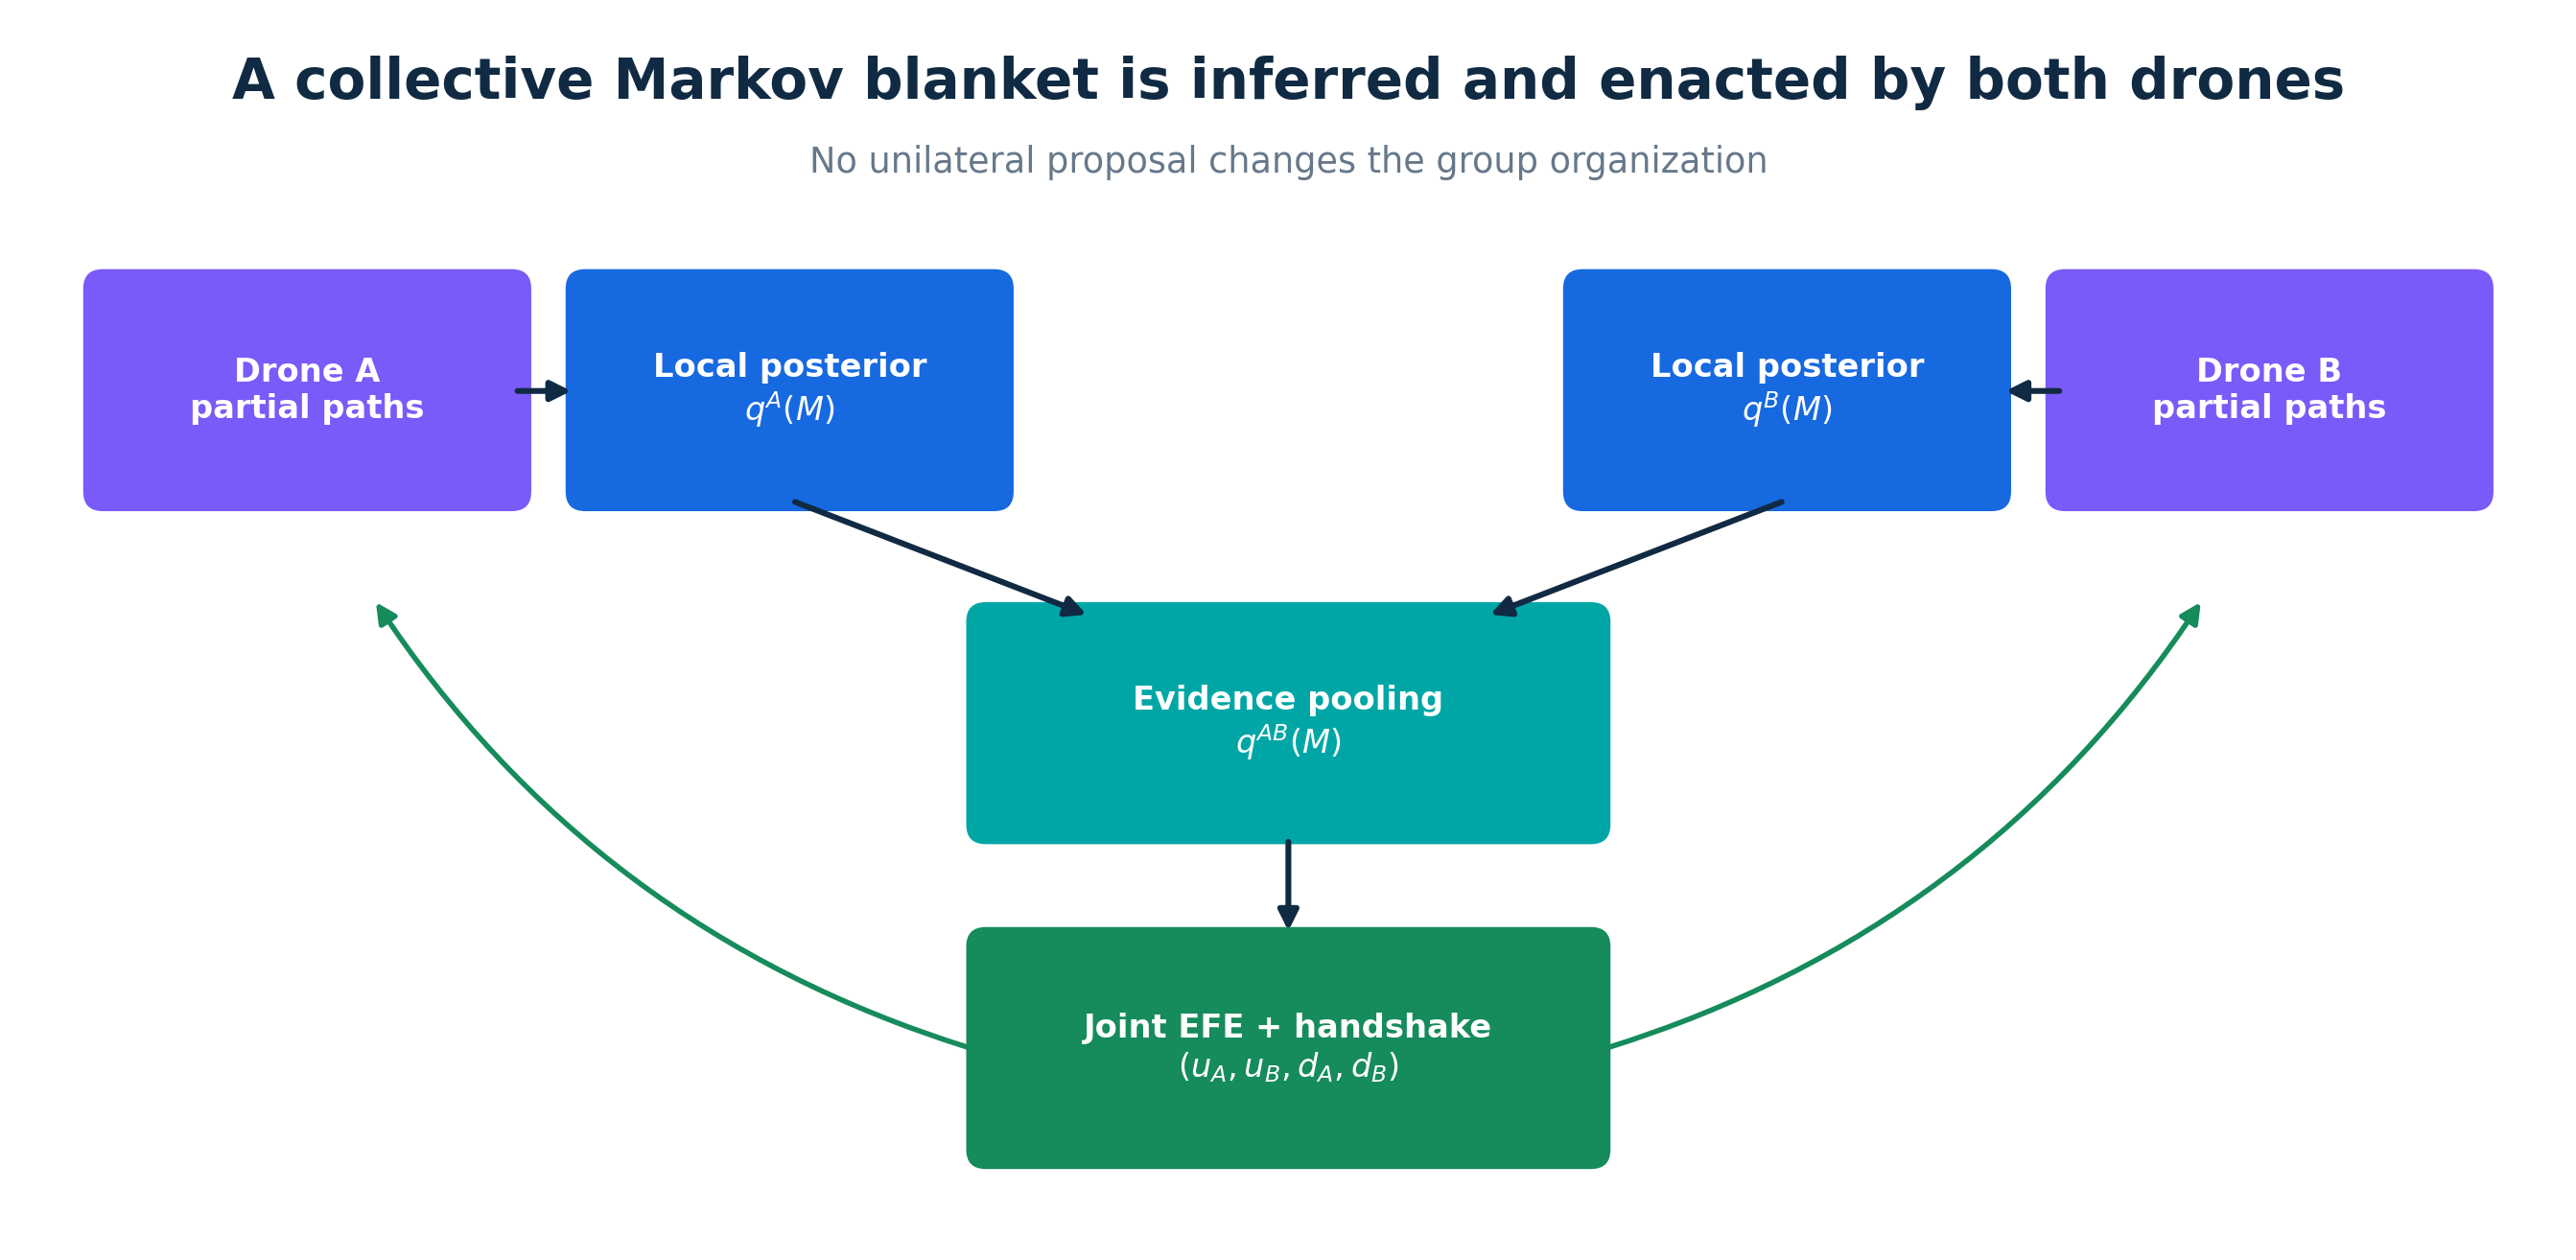
\includegraphics[width=0.94\textwidth]{collective_architecture.png}
 \caption{Collective inference and constitution. Each drone sees only partial
 paths and maintains a local structural posterior. Compressed evidence is
 pooled into a group posterior. A structural change occurs only when both
 agents select the same design proposal under joint EFE.}
 \label{fig:collective-architecture}
\end{figure}

\section{Collective Mathematical Model}

\subsection{Distributed states and candidate partitions}

Let the two vehicles be $a\in\{A,B\}$. The candidate module set remains
$V=\{1,\ldots,8\}$, with ownership map
\begin{equation}
 h(j)=\begin{cases}A,&j\leq4,\\B,&j>4.\end{cases}
 \label{eq:ownership}
\end{equation}
Each owner initially contains one module of each role, but the role labels
are permuted and never supplied to the learners. The collective hypothesis
space is the same constrained set $\Mset$ in
Equation~\eqref{eq:partition-space}; crucially, however, the evidence is
distributed. Drone $A$ observes modules
$V_A=\{1,2,3,4,5,6\}$ and drone $B$ observes
$V_B=\{3,4,5,6,7,8\}$. Their overlap permits alignment, while the private
modules prevent either local record from determining the complete partition.

Let $D_t^a$ be the path fragment available to drone $a$. Local structural
posteriors are
\begin{equation}
 q_t^a(M)=\frac{p(D_t^a\mid M)p_0(M)}
 {\sum_{M'\in\Mset}p(D_t^a\mid M')p_0(M')}.
 \label{eq:local-posterior}
\end{equation}
The agents exchange fixed-size sufficient-statistic messages $m_t^a$, not
ground-truth roles or the physical adjacency matrix. A pooled transition
estimate $\widehat W_t^{AB}$ is fitted from the union of communicated
statistics. To avoid counting the prior twice, the group posterior is
implemented as a logarithmic pool
\begin{equation}
 q_t^{AB}(M)\propto
 \frac{q_t^A(M)q_t^B(M)}{p_0(M)}
 \exp\!\left[\lambda_g\ell(M;\widehat W_t^{AB})\right].
 \label{eq:pooled-posterior}
\end{equation}
All terms range over complete, permutation-aware role assignments. The group
posterior is therefore not a vote over four independent labels.

\subsection{A group-level causal organization}

The collective causal state is
\begin{equation}
 \Corg_t^{AB}=(r_t^{AB},W_t^{AB},L_t^{\times},\rho_t,h),
 \label{eq:group-causal-state}
\end{equation}
where $L_t^{\times}$ contains unscreened links whose endpoints have different
owners. A valid collective blanket screens group-internal paths from exterior
paths conditional on the distributed boundary:
\begin{equation}
 Y_{[0,T]}\indep X^{AB}_{[0,T]}mid
 B^{AB}_{[0,T]},\qquad B^{AB}=(S^{AB},A^{AB}).
 \label{eq:group-factorization}
\end{equation}
The collective factorization gap is
\begin{equation}
 \Gap^{AB}(\Corg_t)=\frac{1}{2\sigma^2}
 \left(\|W^{AB}_{IE}\|_F^2+\|W^{AB}_{EI}\|_F^2\right),
 \label{eq:group-gap}
\end{equation}
computed over the group partition rather than either owner partition.

This definition allows a multiscale fact that is central to the philosophical
argument: a physical module owned by drone $A$ can occupy an active role for
the group, while a module owned by drone $B$ can occupy a sensory role for the
same group. Hardware ownership and blanket membership are different
relations. The group boundary cuts across the two chassis.

\subsection{Bilateral constitution}

Each drone proposes a structural action $d_t^a\in\mathcal D^{AB}$.
Cross-owner shielding removes a bypass between modules on different bodies;
cross-owner routing exchanges two modules' group-level causal ports. The
collective transition is
\begin{equation}
 \Corg_{t+1}^{AB}=
 \begin{cases}
  \Tmap^{AB}(\Corg_t^{AB},d_t^A,\omega_t),
  & d_t^A=d_t^B\neq d^0,\\
  \Tmap^{AB}(\Corg_t^{AB},d^0,\omega_t),&\text{otherwise.}
 \end{cases}
 \label{eq:handshake}
\end{equation}
Thus
\begin{equation}
 \Tmap^{AB}(\Corg,d,d^0,\omega)
 =\Tmap^{AB}(\Corg,d^0,d,\omega)
 =\Tmap^{AB}(\Corg,d^0,d^0,\omega),
 \label{eq:no-unilateral-effect}
\end{equation}
while two matching non-null proposals can change $W^{AB}$ or $r^{AB}$. This
handshake is not meant as a universal model of social agreement. It is an
experimental identifiability device: it makes collective causal efficacy
irreducible to one privileged agent.

\subsection{Shared payload and formation dynamics}

Let $y_t^A$ and $y_t^B$ be lateral positions. The task variables are shared
payload displacement and formation error,
\begin{equation}
 p_t=\tfrac12(y_t^A+y_t^B),\qquad
 f_t=(y_t^B-y_t^A)-f^*,
 \label{eq:payload-formation}
\end{equation}
where $f^*$ is the preferred separation. The two control inputs affect the
center and relative modes:
\begin{align}
 p_{t+1}&=\alpha_p p_t+\delta_p(\bar u_t+w_t)+\xi_t^p,\\
 f_{t+1}&=\alpha_f f_t+\delta_f(u_t^B-u_t^A)+\xi_t^f,
 \label{eq:collective-dynamics}
\end{align}
with $\bar u_t=(u_t^A+u_t^B)/2$. Sensory precision changes uncertainty in
both estimates; active precision changes effective actuation. Cross-owner
breaches add correlated disturbances and energetic compensation. The group
viability score is a bounded function of payload RMSE, formation RMSE,
collision, energy, factorization gap, and routed boundary precision.

\subsection{Joint expected free energy and agreement}

A collective policy is
$\pi^{AB}=(u^A,u^B,d^A,d^B)$. The implemented group EFE is
\begin{align}
 G_t^{AB}(\pi^{AB})
 &=R_t^{\mathrm{payload}}+R_t^{\mathrm{formation}}
   +R_t^{\mathrm{energy}}+\alpha\mathcal A_t^{AB}\\
 &\quad+c(d^A)+c(d^B)
 -\beta_M\E[\Delta Q_{\mathrm{arch}}^{AB}]
 -\beta_I\MI(M;o_{t+1}^{AB}\mid\pi^{AB})
 +\kappa\mathbf1[d^A\neq d^B].
 \label{eq:collective-efe}
\end{align}
The final term prices disagreement because unmatched proposals consume a
design opportunity but cannot change the organization. Each drone evaluates
candidate pairs using $q_t^{AB}$ and the learned family-level efficacy model,
then samples from a shared softmax
\begin{equation}
 q(\pi^{AB})\propto\exp[-G_t^{AB}(\pi^{AB})/\gamma_g].
 \label{eq:group-policy}
\end{equation}
Agreement is therefore endogenous to policy selection rather than imposed
after two independent decisions.

\section{Collective Experimental Design}

\subsection{Tasks}

\textbf{Assembly.} The pair begins with cross-owner internal--external bypass
links. It must infer which cross-body couplings violate the group partition
and agree on the corresponding shields. This constructs a group boundary that
was absent at mission start.

\textbf{Repair.} The pair begins with a clean group boundary. At a random time
a cross-owner bypass opens. A nonspecific integrity alarm enables structural
action but does not identify the link or reveal role labels. The drones must
localize and close the breach before mission end.

\textbf{Reconfiguration.} A currently useful boundary module loses precision
while a precise external module owned by the other drone becomes available.
The factorization gap remains zero, so generic shielding cannot solve the
task. The agents must agree on the appropriate cross-owner port exchange.
This is the strongest discrimination between purposive design and random
structural action.

\subsection{Conditions and controls}

\begin{table}[t]
\centering
\small
\begin{tabularx}{\textwidth}{>{\bfseries}lX}
\toprule
Condition & Operational definition \\
\midrule
Collective constitutive & Pooled posterior, joint EFE, bilateral handshake,
and physically effective group-level design. \\
Collective diagnostic & Same inference, messages, and nominal agreement, but
design cannot alter $\Corg^{AB}$. \\
Individual constitutive & Each drone acts from its local posterior; matching
proposals can act, but there is no pooled group model. \\
Fixed team & Shared controller with no structural action and a fixed
engineered interface. \\
Communication only & Same aggregate message budget, used for raw state
sharing without a role posterior or boundary model. \\
Random joint & Bilaterally matched structural actions sampled without EFE. \\
Oracle collective & Ground-truth breach or precision mismatch selects the
bilateral action; this is an upper bound, not a realizable learner. \\
\bottomrule
\end{tabularx}
\caption{Part~II conditions. Communication-only is the critical control for
the possibility that bandwidth, rather than blanket inference, produces the
strategic advantage.}
\label{tab:collective-conditions}
\end{table}

The frozen protocol uses 20 held-out paired seeds for each of seven
conditions and three tasks: 420 missions of 90 steps. The seed offset (2000),
software versions, and full mission-level observations are stored with the
results. Primary outcomes are task success and group architecture score.
Secondary outcomes are group viability, payload and formation RMSE, energy,
final factorization gap, role and blanket-set accuracy, exact partition
recovery, agreements, and realized causal changes.

\section{Collective Results}

\subsection{Constitution and strategic advantage}

The collective constitutive agent succeeds in 80\% of assembly missions,
90\% of repair missions, and 100\% of reconfiguration missions
(Figure~\ref{fig:collective-benchmark}). Both the collective diagnostic and
equal-bandwidth communication controls score 0\% on all three tasks. Against
communication only, the paired success advantages are
$0.80\pm0.092$, $0.90\pm0.069$, and $1.00\pm0.000$; group viability advantages
are $0.114\pm0.018$, $0.052\pm0.004$, and $0.111\pm0.004$.

\begin{figure}[p]
 \centering
 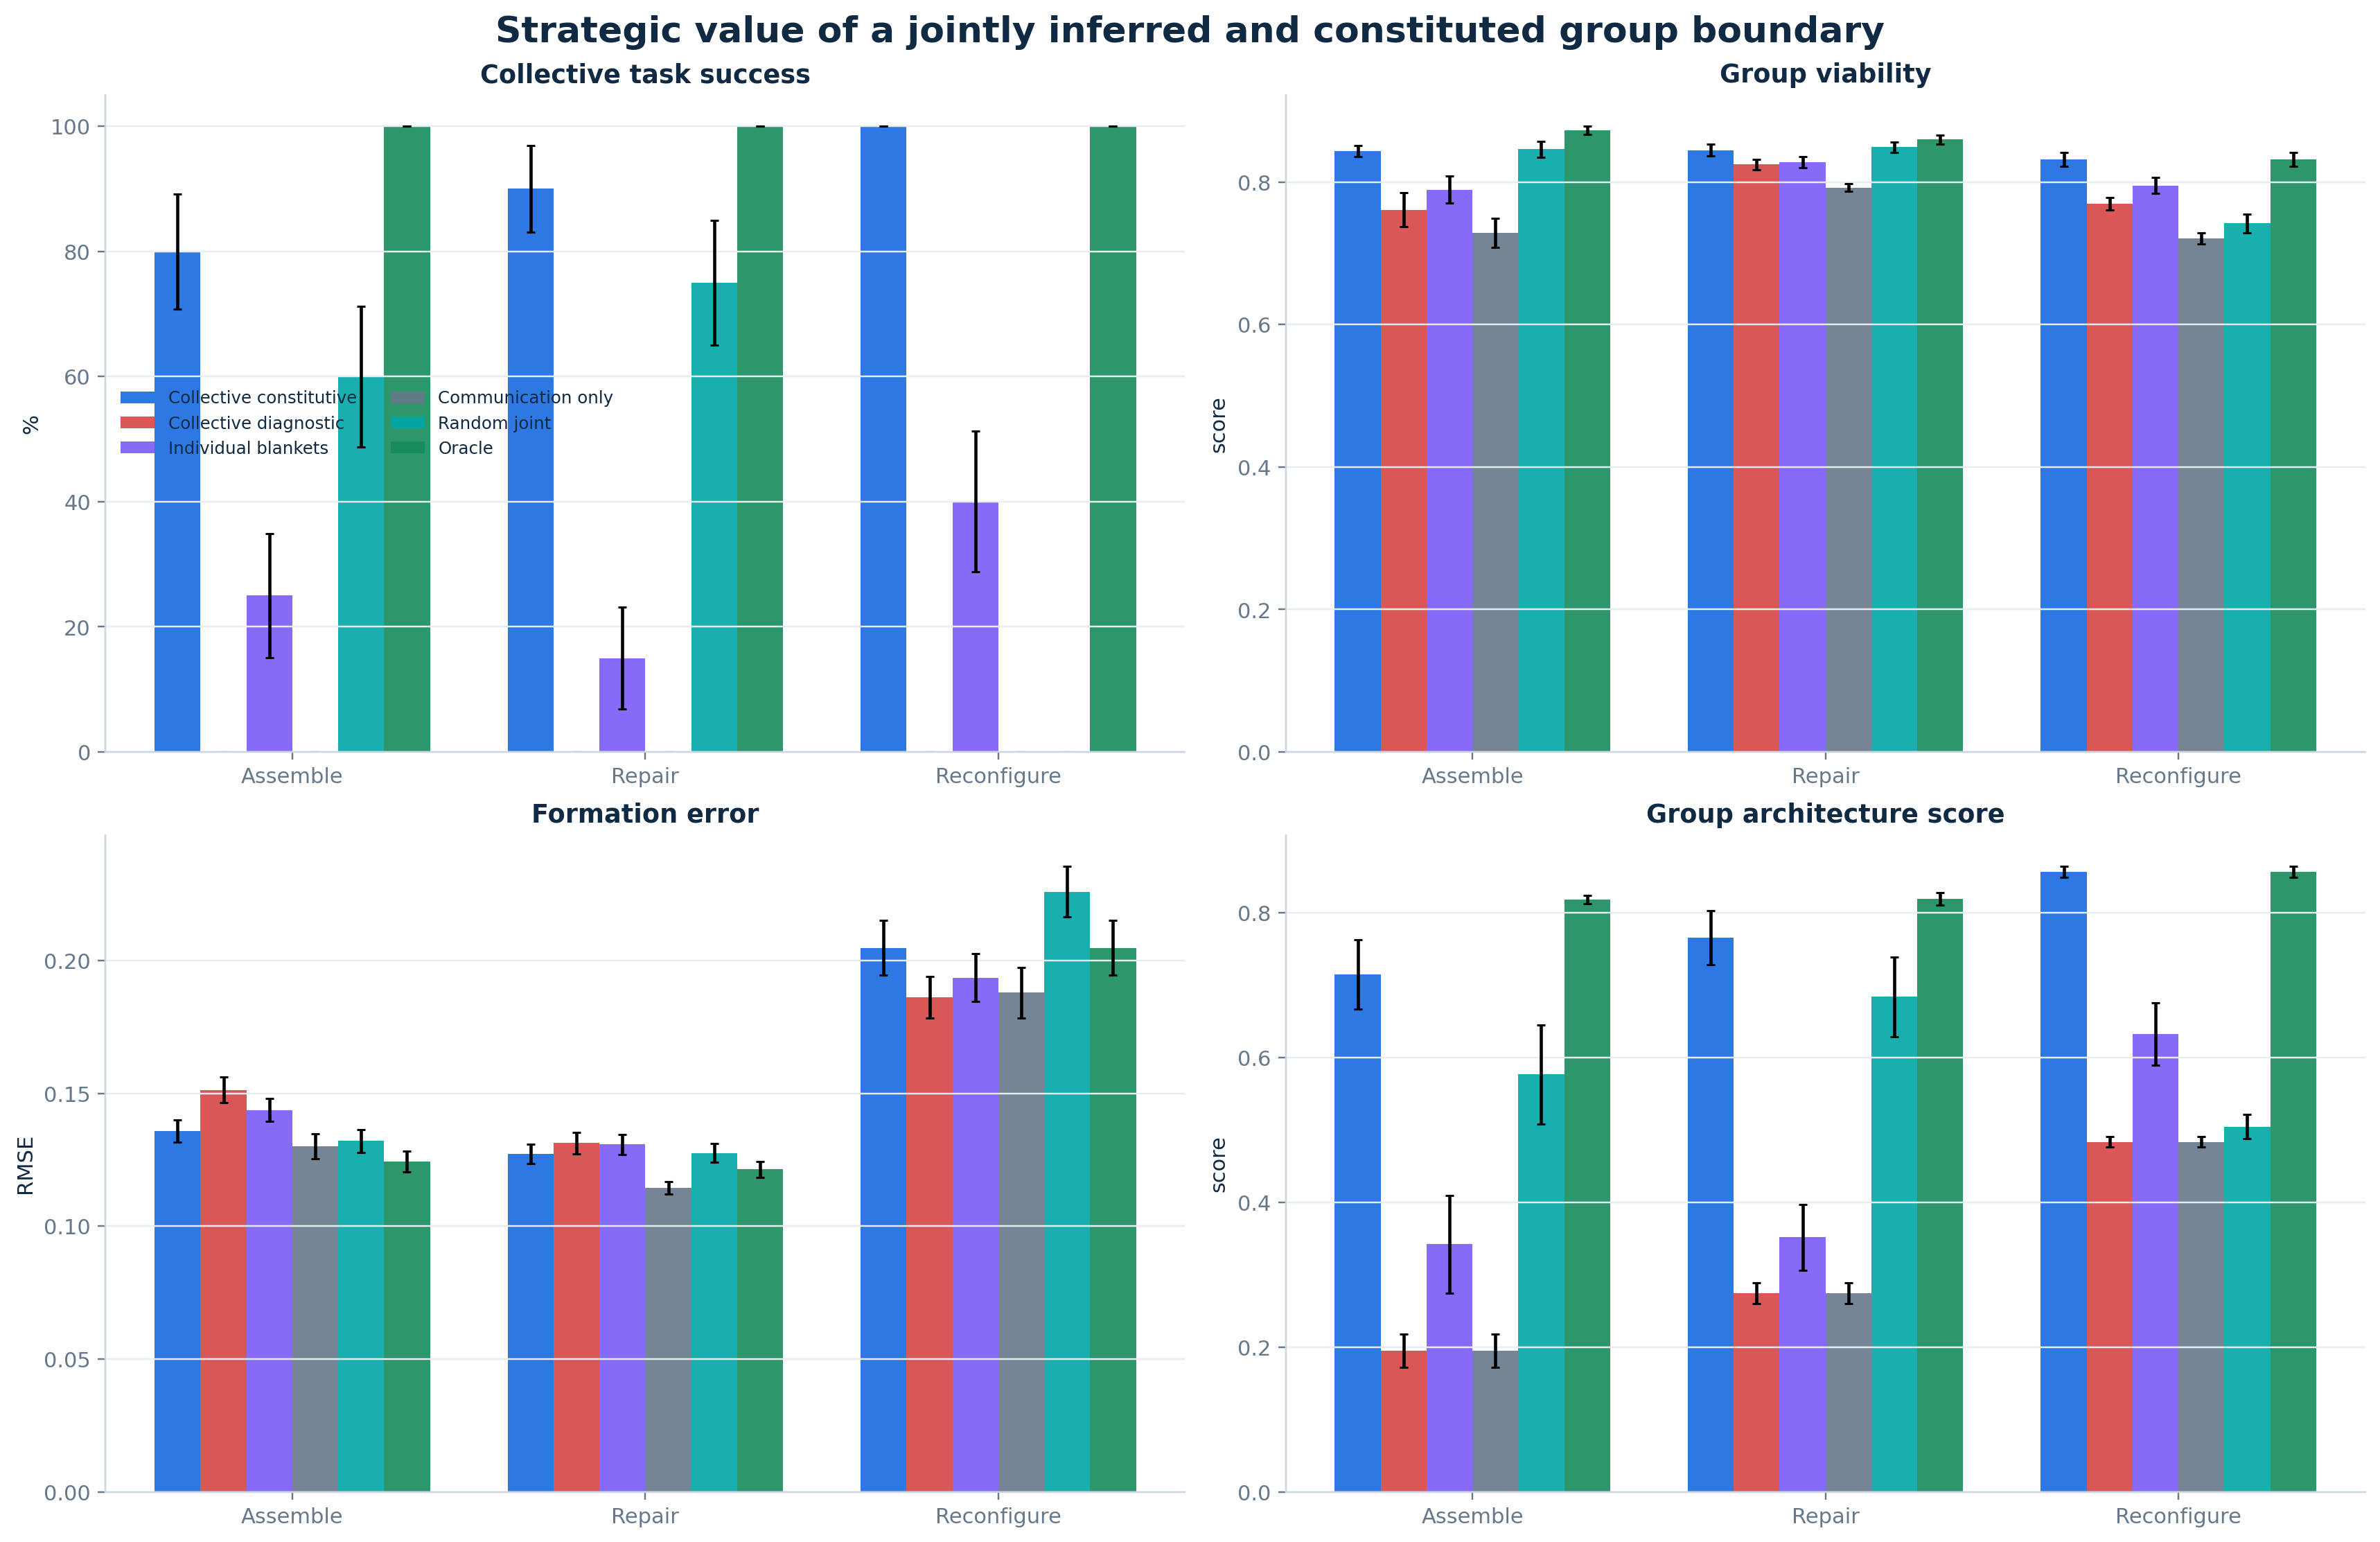
\includegraphics[width=\textwidth]{collective_benchmark.png}
 \caption{Collective benchmark. Error bars are seed-level standard errors.
 Success requires the targeted group organization, not merely collision-free
 motion. The oracle marks the attainable ceiling.}
 \label{fig:collective-benchmark}
\end{figure}

Compared with individual constitutive agents, the collective success
advantages are $0.55\pm0.114$ in assembly, $0.75\pm0.099$ in repair, and
$0.60\pm0.112$ in reconfiguration. The corresponding architecture-score
advantages are $0.373\pm0.071$, $0.414\pm0.056$, and $0.224\pm0.043$. These
comparisons answer RQ2 narrowly: pooled structural evidence plus bilateral
design outperforms local blankets under the simulated partial-observability
regime.

\subsection{Why messaging alone is not enough}

The communication-only agents receive the same aggregate bandwidth and often
obtain competitive payload or formation estimates. Nevertheless they cannot
close a bypass or reroute a boundary port because their messages are not
organized as evidence about a candidate partition and their controller has no
causal boundary target. Figure~\ref{fig:strategic-advantage} shows the paired
viability comparison. Almost every seed lies above the identity relation in
favor of collective boundary design.

\begin{figure}[t]
 \centering
 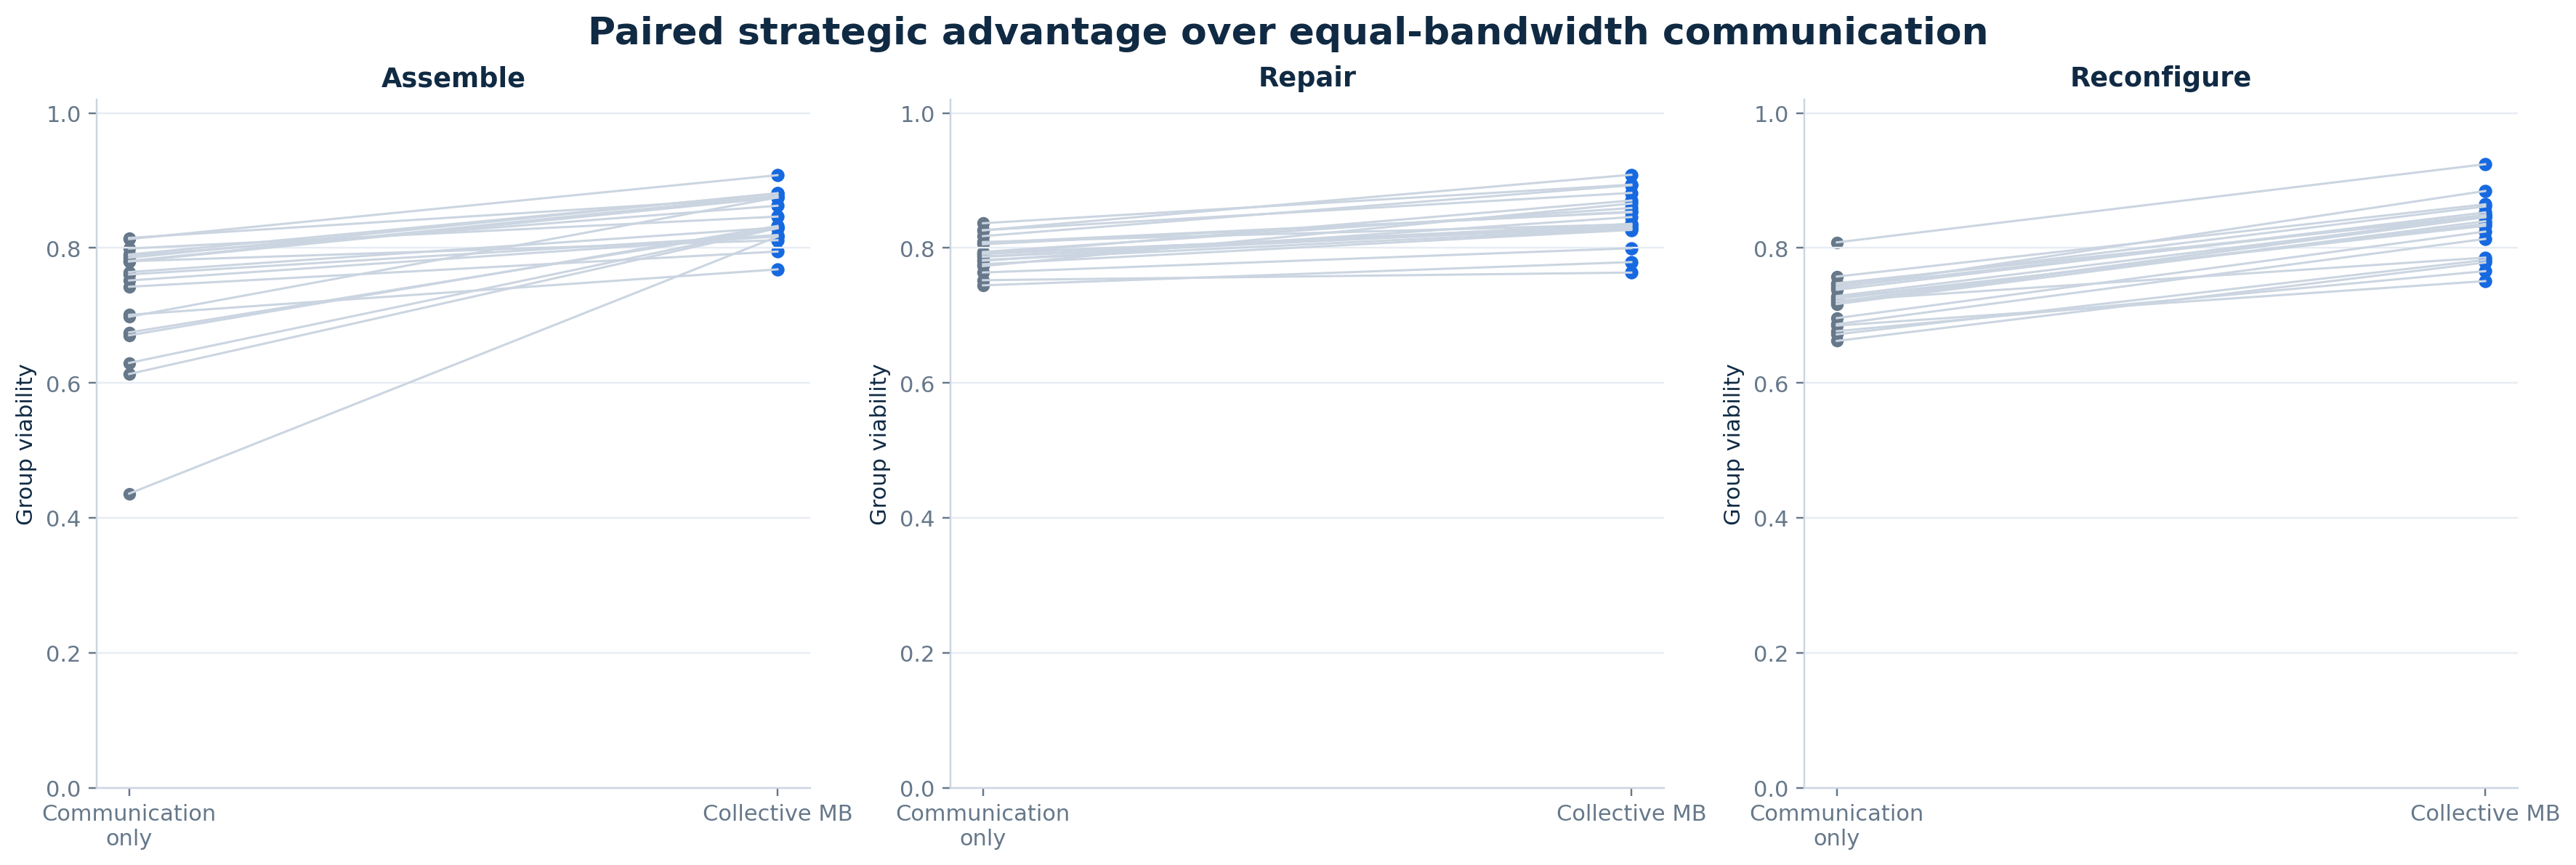
\includegraphics[width=\textwidth]{collective_strategic_advantage.png}
 \caption{Paired strategic advantage over equal-bandwidth communication.
 Lines connect the same exogenous seed. The comparison isolates the value of
 representing and constituting a group boundary from the value of sharing
 data as such.}
 \label{fig:strategic-advantage}
\end{figure}

The distinction is not that communication is unnecessary. Evidence pooling
is itself communicative. The point is that bandwidth is organized by a model
of causal roles and connected to actions that can change those roles.
Collective individuation is a use of communication, not an alternative to it.

\subsection{Random constitution and directed transformation}

Random joint action succeeds in 60\% of assembly and 75\% of repair missions.
This is expected in a small action space: repeated matched shielding can
eventually hit a breach. Random action nevertheless succeeds in 0\% of
reconfiguration missions, where the target is one precision-improving
cross-owner swap among multiple causally valid partitions. Thus the data do
not show that EFE is necessary for every causal modification. They show that
EFE supplies selectivity when several structural changes are possible and
only one realizes the preferred interface.

\begin{figure}[p]
 \centering
 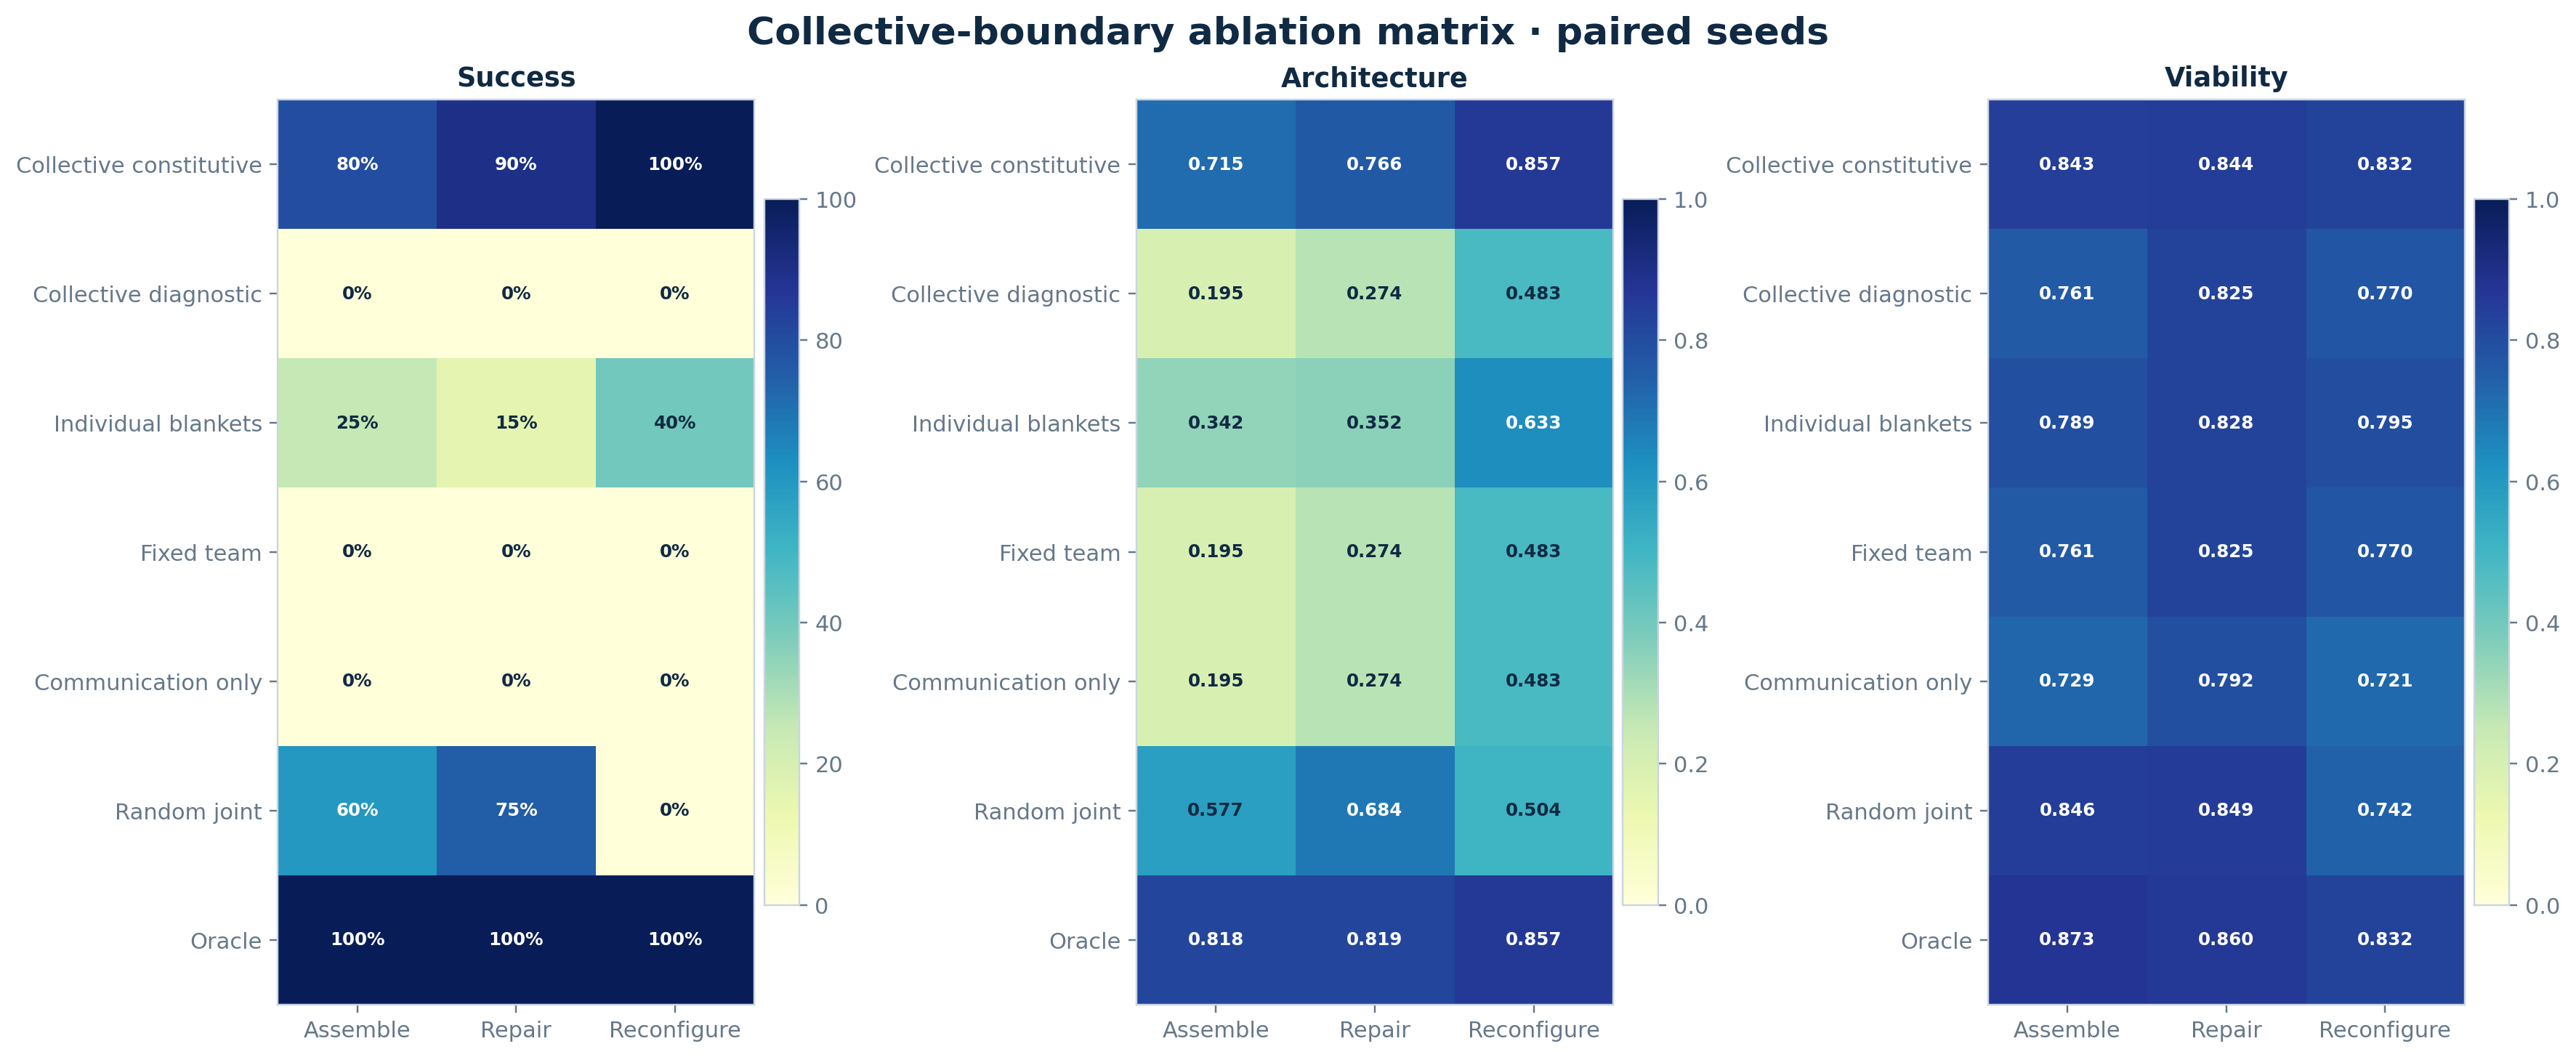
\includegraphics[width=\textwidth]{collective_ablation_matrix.png}
 \caption{Collective ablation matrix. The reconfiguration column is the
 discriminating test for purposive boundary design: factorization alone does
 not choose among multiple zero-gap boundaries.}
 \label{fig:collective-ablation}
\end{figure}

\subsection{Time-resolved examples}

Figure~\ref{fig:collective-examples} displays one successful mission per task.
In assembly the factorization gap collapses after agreed shielding. In repair
the gap rises at the exogenous breach and returns to zero only after a
bilateral action. In reconfiguration the gap remains zero throughout, but the
agreed swap improves the routed precision needed for payload and formation
control. These different signatures are why construct, stabilize, and
transform cannot be collapsed into a single ``adaptation'' score.

\begin{figure}[p]
 \centering
 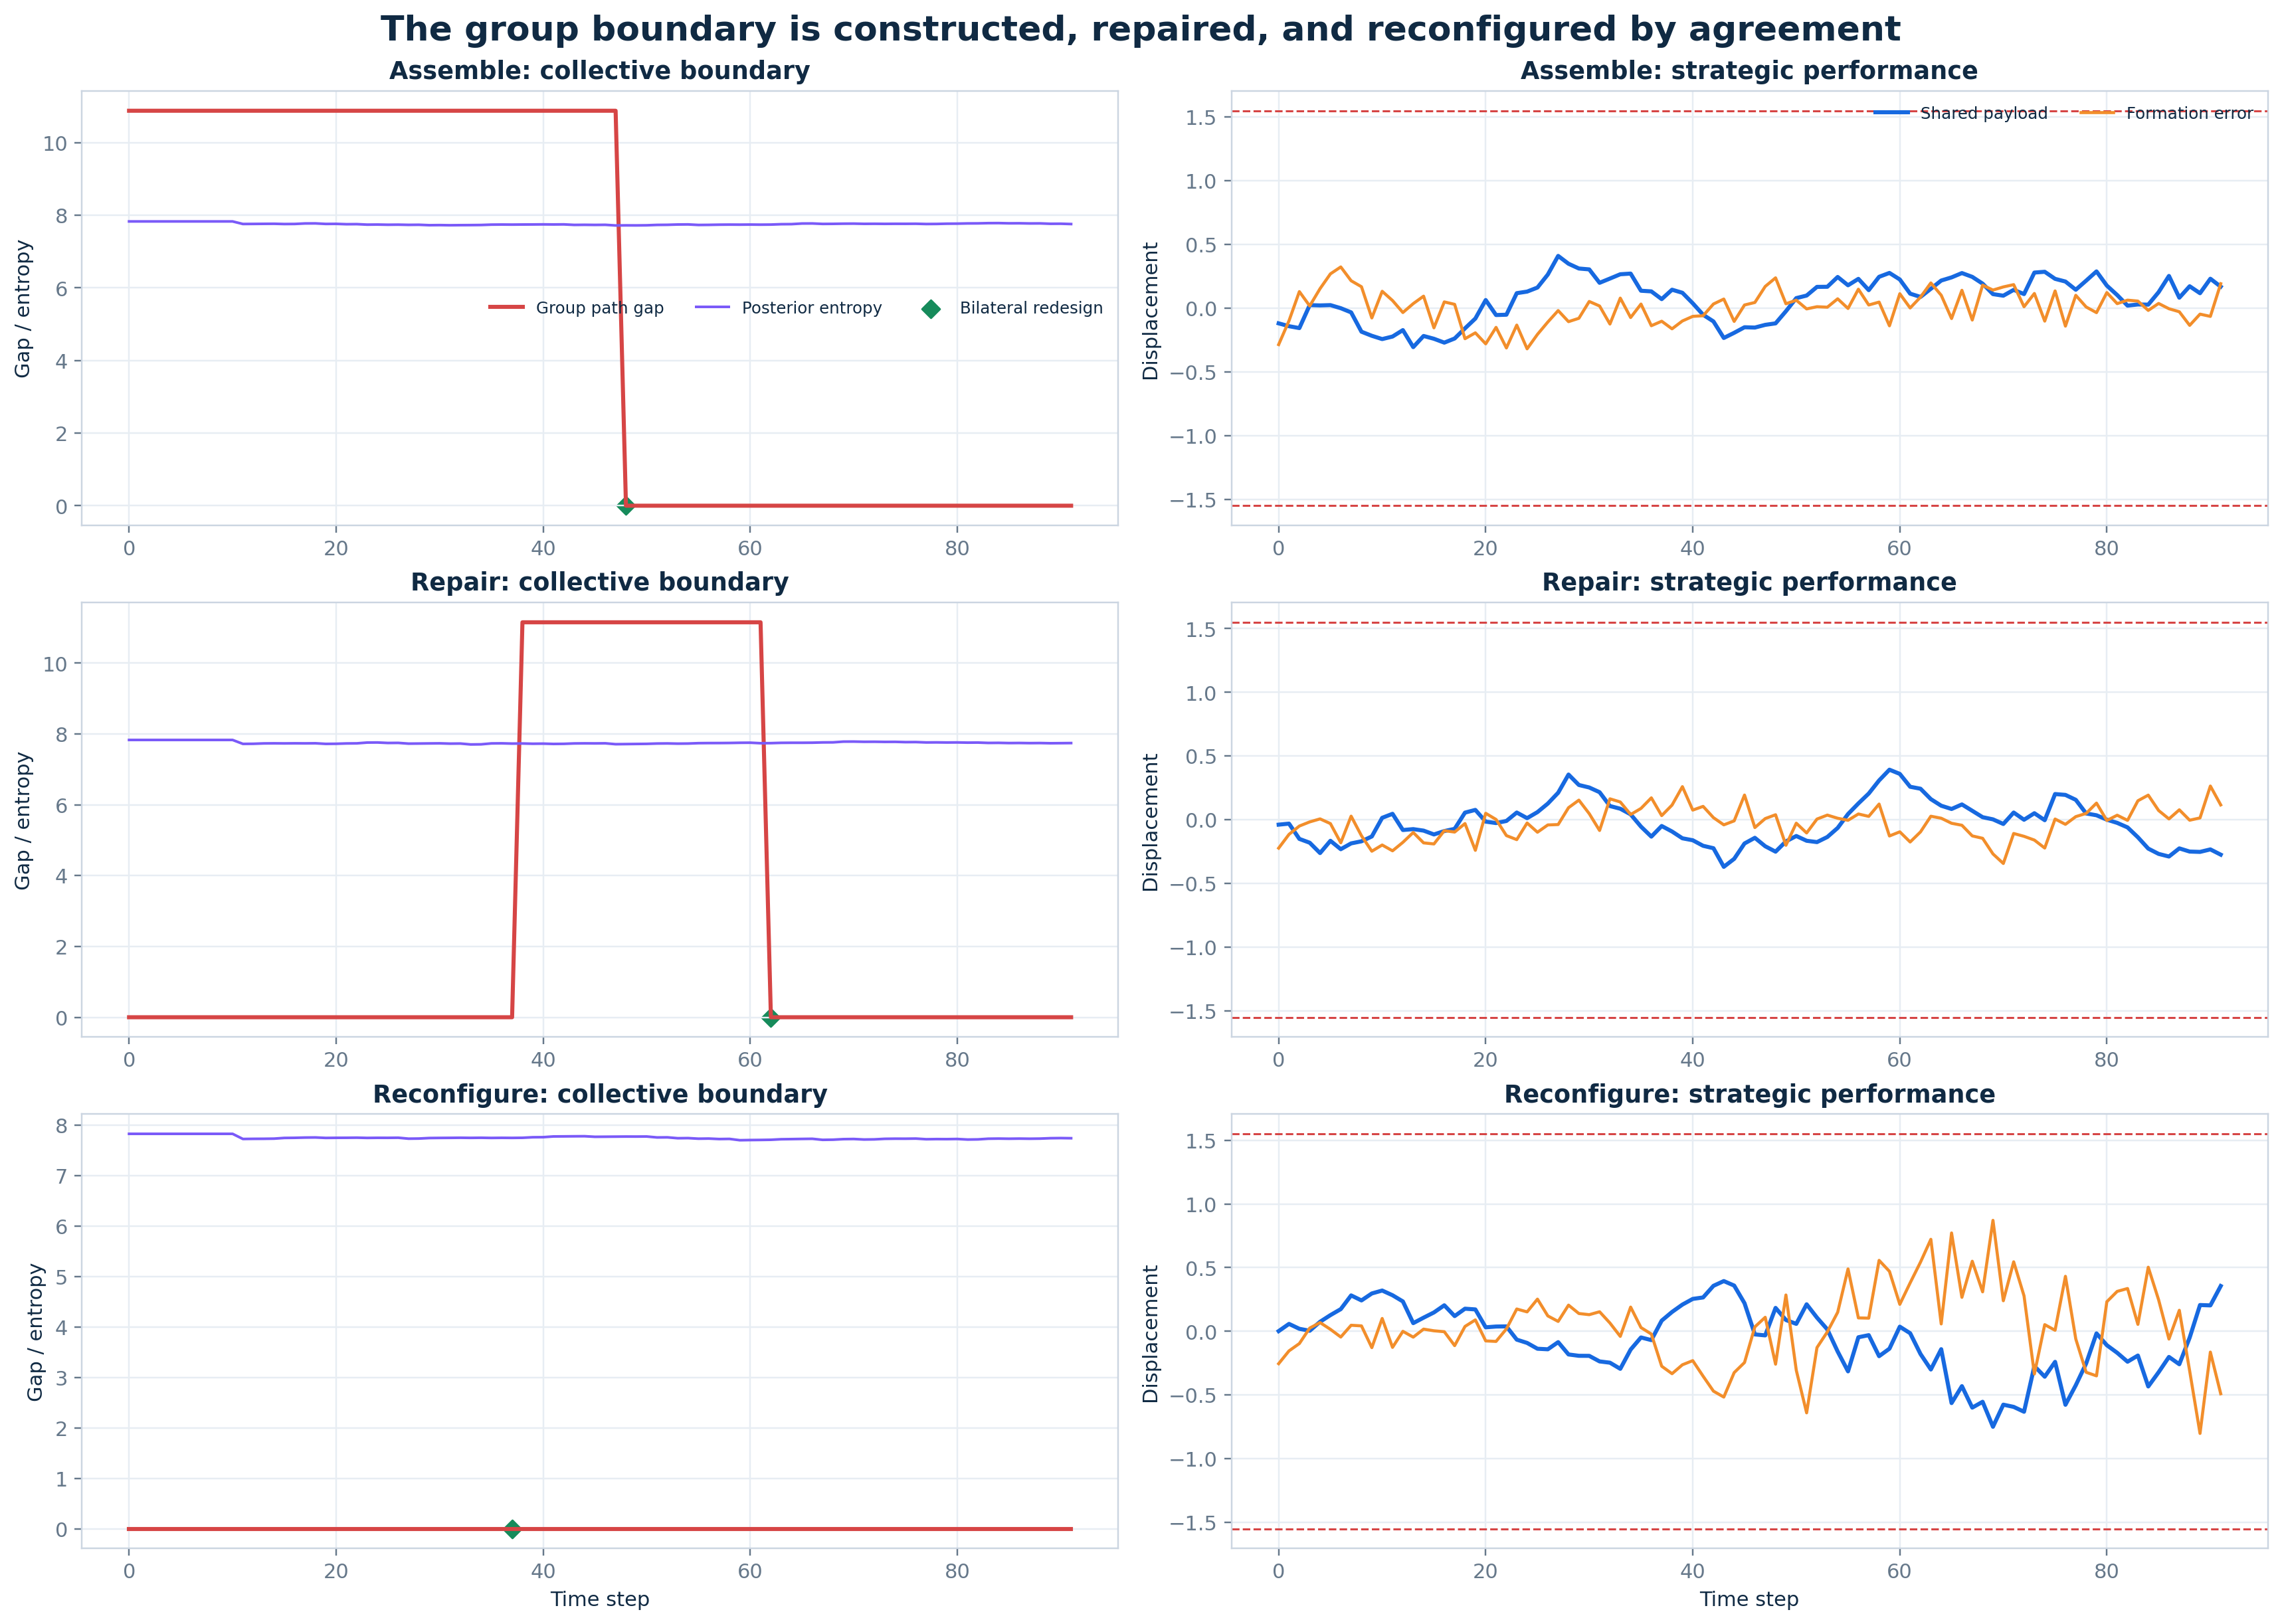
\includegraphics[width=\textwidth]{collective_examples.png}
 \caption{Representative collective missions. Green diamonds mark bilateral
 changes to the group organization. Red traces are group factorization gaps;
 violet traces are posterior entropies; right panels show shared payload and
 formation trajectories.}
 \label{fig:collective-examples}
\end{figure}

\begin{table}[p]
\centering
\scriptsize
\setlength{\tabcolsep}{3.5pt}
\begin{tabular}{llrrrrrr}
\toprule
Condition & Task & Success & Viability & $Q_{arch}^{AB}$ & Payload RMSE & Formation RMSE & Energy \\
\midrule
Collective constitutive & Assemble & 80\% & .843 & .715 & .183 & .136 & 8.69 \\
 & Repair & 90\% & .844 & .766 & .183 & .127 & 8.62 \\
 & Reconfigure & 100\% & .832 & .857 & .189 & .205 & 8.69 \\
\addlinespace
Collective diagnostic & Assemble & 0\% & .761 & .195 & .276 & .151 & 12.84 \\
 & Repair & 0\% & .825 & .274 & .198 & .131 & 10.08 \\
 & Reconfigure & 0\% & .770 & .483 & .180 & .186 & 8.17 \\
\addlinespace
Individual constitutive & Assemble & 25\% & .789 & .342 & .244 & .144 & 11.44 \\
 & Repair & 15\% & .828 & .352 & .197 & .131 & 9.81 \\
 & Reconfigure & 40\% & .795 & .633 & .183 & .194 & 8.38 \\
\addlinespace
Communication only & Assemble & 0\% & .729 & .195 & .200 & .130 & 19.29 \\
 & Repair & 0\% & .792 & .274 & .107 & .114 & 15.93 \\
 & Reconfigure & 0\% & .721 & .483 & .118 & .188 & 15.17 \\
\addlinespace
Random joint & Assemble & 60\% & .846 & .577 & .177 & .132 & 8.61 \\
 & Repair & 75\% & .849 & .684 & .179 & .128 & 8.32 \\
 & Reconfigure & 0\% & .742 & .504 & .208 & .226 & 10.03 \\
\addlinespace
Oracle collective & Assemble & 100\% & .873 & .818 & .158 & .124 & 6.64 \\
 & Repair & 100\% & .860 & .819 & .172 & .121 & 7.52 \\
 & Reconfigure & 100\% & .832 & .857 & .189 & .205 & 8.69 \\
\bottomrule
\end{tabular}
\caption{Selected complete Part~II outcomes. Means are over 20 paired seeds.
The fixed-team condition is numerically identical to collective diagnostic
for the reported variables and is retained in the archived CSV.}
\label{tab:collective-results}
\end{table}

\FloatBarrier

\part{Synthesis}
\section{Discussion}

\subsection{What the model now demonstrates}

Part~I establishes more than detection or tracking in its simulated domain.
First, a drone-selected action changes the physical causal organization under
an otherwise fixed exogenous realization. Second, that change can remove a
path-law coupling or reassign a physical module to a different interface
role. Third, the change improves a preregistered architecture score and, in
the construction and transformation settings, viability. Fourth, the effect
disappears in the diagnostic-only control.

These points operationalize Possati's inversion. The agent does not merely
discover where a boundary already is. It uses the discovered organization to
select material operations that make another boundary true. Construction,
stabilization, and transformation are separated because they are different
claims: closing initial bypasses, repairing a later breach, and changing a
valid boundary because another valid boundary better supports the task.

Part~II adds a distinct result. The successful unit of structural action is
not either vehicle by itself. Local learners have incomplete evidence;
unilateral proposals are causally inert; and the target partition crosses
hardware ownership. The enacted organization improves group viability over
an equal-bandwidth controller and improves targeted success over two local
constitutive agents. In this bounded sense, the pair becomes a single
operational agent for the shared task: it acquires a joint inferential
interior and a jointly controlled interface.

\subsection{Why the book connection is substantive}

The model clarifies the philosophical claim in three ways. First, a Markov
blanket is treated as a structuring of possible state paths, not as an object
surface. Second, inversion is doubled: Bayesian inversion estimates the
current structure, while design inversion acts on the world so that a
preferred structure becomes realized. Third, precision, curiosity, and
prediction cease to be exclusively mental or computational notions. They
become properties of material selection, intervention, and routing.

This is the precise point at which Possati differs from accounts that use
active inference to optimize an artifact inside a fixed system boundary.
Niche construction changes environmental states; interaction design changes
the observations available to a user; explainable active inference changes
access to internal beliefs. Possati's strong proposal concerns the causal
partition that makes ``internal,'' ``sensory,'' ``active,'' and ``external''
roles possible in the first place. V5 is a deliberately minimal realization
of that claim.

The collective extension sharpens the book's thesis. If boundaries were
fixed surfaces, two drones could only cooperate across already constituted
interfaces. If blankets are organizations of paths, however, cooperation can
itself have a boundary that is discovered and materially sustained. The
interface is then not simply between drone $A$ and drone $B$; it can run
through both of them, separating group-internal dynamics from the shared
environment. Possati's inversion becomes multiscale: design does not only
alter what an existing individual senses and does, but can alter which
individual is the relevant unit of sensing and doing.

\subsection{Does the pair literally become one drone?}

The experiment warrants an operational, not an unrestricted ontological,
answer. It supplies four pieces of evidence for group-level individuation:
a nontrivial collective partition, distributed epistemic access, irreducibly
bilateral causal control, and a strategic consequence of maintaining the
partition. These criteria exclude mere co-location and simple data exchange.
They do not prove phenomenal unity, biological autonomy, indefinite
self-maintenance, or persistence across arbitrary tasks.

The most defensible formulation is therefore: the two vehicles instantiate
one \emph{task-relative control unit} over the mission horizon. Whether that
unit should count as one artifact without qualification depends on further
criteria---material integration, counterfactual robustness, persistence,
normative closure, and the capacity to recreate its own enabling components.
The present Markov-blanket evidence is neither trivial nor metaphysically
decisive.

\subsection{Alternative explanations and the role of the controls}

Five alternatives are addressed experimentally. Better results are not due
only to model updating, because the diagnostic control updates without
constituting. They are not due only to communication, because bandwidth is
matched. They are not due only to structural actuation, because random joint
action fails targeted transformation. They are not reducible to two
independent local blankets, because the individual condition lacks the full
evidence and performs worse. Finally, they are not due to an exogenous role
switch: disturbances alter couplings or precision, while the role exchange
is selected by the agents.

Not every alternative is excluded. The simulator and success criteria share
the same formal vocabulary; the controller is therefore evaluated in a world
whose relevant regularities it can represent. The action set is small, the
message topology is engineered, and both agents use the same model class.
Robustness to model misspecification and heterogeneous learners remains open.

\subsection{What remains unproven}

Six limitations delimit the result. First, the eight candidate modules are
declared. The system does not discover an unbounded ontology. Second, the
action repertoire is engineered: shielding and port exchange are known
affordance types even though their success is learned. Third, the
linear-Gaussian gap in Equation~\eqref{eq:gap} is exact only for the simulator's
chosen local path-law comparison. Nonlinear, partially observed hardware
requires richer estimators. Fourth, the EFE score uses engineering weights
and a short horizon. It demonstrates the conjunction of pragmatic,
ambiguity, and epistemic terms, not a unique first-principles controller.
Fifth, the collective handshake is a designed institution rather than an
emergent communication protocol. Sixth, all results come from a
linear-Gaussian simulator and 20 seeds per cell; they establish internal
proof-of-concept validity, not ecological generality.

The learned intervention model is also intentionally small. A stronger V6
would learn action-conditioned changes to the full transition matrix,
represent uncertainty over hardware affordances, and evaluate counterfactual
path laws over longer horizons. A hardware experiment would require safe
reconfigurable sensor buses, redundant actuators, online causal estimation,
and a conservative supervisory layer.
 A stronger collective version would also learn who participates in the
group, the communication graph, and the conditions under which the group
should dissolve.

\section{Conclusion}

The decisive question was whether ``boundary design'' named a causal
operation or only a redescription. V5 makes that question testable by
separating the inferred blanket from the physical organization, allowing
design actions to modify the latter, and comparing them against identical
diagnostic actions that cannot. Within the declared simulator, the result is
positive across construction, stabilization, and transformation. The second
experiment shows that the same logic can cross physical bodies: two drones
can pool evidence, agree on a structural operation, and enact a task-relative
group boundary that improves strategic performance. The proper claim is
narrow but no longer metaphorical. A single drone can redesign its
statistical interface, and a pair can constitute an operational interface
that neither can maintain alone.

\section*{Reproducibility Statement}

The repository contains the complete source, unit tests, fixed seed offsets,
mission-level CSVs, paired effects, mediation output, run metadata, and figure
generation code. Part~I is reproduced with
\texttt{python run\_experiment.py --seeds 20 --seed-offset 1000 --workers 6};
Part~II uses
\texttt{python run\_collective\_experiment.py --seeds 20 --seed-offset 2000
--workers 6}. The diagnostic-only contrasts, equal-bandwidth communication
control, paired seeds, and all three tasks must be retained in replication.

\appendix
\part*{Technical Appendices}
\addcontentsline{toc}{part}{Technical Appendices}

\section{Path-Space Factorization and the Linear Gap}

This appendix states the limited derivation behind
Equation~\eqref{eq:gap}. Consider two path coordinates $X$ and $Y$ after
conditioning on a proposed blanket path $B$. Let $P$ denote a diffusion with
direct residual cross-drift $g_t=(W_{XY}Y_t,W_{YX}X_t)$ and let $P^0$ denote
the same diffusion with that cross-drift removed. If both laws share
nonsingular diffusion matrix $\sigma I$ and satisfy the usual absolute
continuity and integrability conditions, Girsanov's theorem gives
\begin{equation}
 \KL(P\|P^0)=\frac{1}{2\sigma^2}
 \E_P\int_0^T \|g_t\|_2^2\,\mathrm dt.
 \label{eq:girsanov-kl}
\end{equation}
For standardized coordinates with unit second moment and a locally constant
drift matrix,
\begin{align}
 \frac1T\KL(P\|P^0)
 &\approx \frac{1}{2\sigma^2}
 \E\bigl[\|W_{XY}Y\|_2^2+\|W_{YX}X\|_2^2\bigr]\\
 &\approx \frac{1}{2\sigma^2}
 \left(\|W_{XY}\|_F^2+\|W_{YX}\|_F^2\right).
 \label{eq:frobenius-gap}
\end{align}
The right-hand side is the implemented $\Gap$. It vanishes when the proposed
blanket screens direct cross-drift in the simulator. It is a local
relative-entropy-rate proxy, not an estimator of arbitrary nonlinear
conditional mutual information. Autocorrelation, latent common causes, or
state-dependent diffusion would require a richer path-law model.

For the stabilization task, the paired effect is identifiable because the
same disturbance realization is used in both arms. Let
$\omega_{0:T}^{(s)}$ be seed $s$'s exogenous stream. Then
\begin{equation}
 \delta_s=\Gap\!\left(\Corg_T^{\mathrm{constitutive}}
 (\omega^{(s)})\right)-
 \Gap\!\left(\Corg_T^{\mathrm{diagnostic}}
 (\omega^{(s)})\right)
 \label{eq:paired-gap}
\end{equation}
isolates whether the selected design operation is permitted to change the
causal organization. The reported standard error is
$\mathrm{sd}(\delta_s)/\sqrt{20}$.

\section{Exact Partition Posterior and Permutation Awareness}

The eight-module role space is generated by nested combinations. Choose two
modules for $\Irole$, two from the remainder for $\Srole$, two for $\Arole$,
and assign the final two to $\Erole$. This yields
\begin{equation}
 \binom{8}{2}\binom{6}{2}\binom{4}{2}\binom{2}{2}=2520
 \label{eq:enumeration}
\end{equation}
hypotheses. Because the members within a role are exchangeable, evaluation
compares role sets rather than arbitrary node order. Exact partition accuracy
is
\begin{equation}
 \mathbf1\!\left[\arg\max_{M\in\Mset}q_T(M)=M_T^{\mathrm{true}}\right],
 \label{eq:exact-partition}
\end{equation}
and blanket-set accuracy averages classification of membership in
$B=S\cup A$. Exact recovery is reported separately from task success because
an agent can select a useful intervention under posterior uncertainty without
recovering every role label.

The structural template score uses magnitude to detect adjacency and learned
control/noise terms to orient the cycle. This prevents a purely symmetric
graph match from arbitrarily exchanging sensory and active labels. A hazard
mixture
\begin{equation}
 \widetilde q_t(M)=(1-h)q_t(M)+h/|\Mset|
 \label{eq:hazard}
\end{equation}
keeps alternatives alive after structural change. In the collective model,
the same hypothesis index is shared between local and pooled posteriors, so
logarithmic pooling cannot combine incompatible label spaces.

\section{Algorithms}

\subsection{Individual constitutive inversion}

\begin{enumerate}[leftmargin=1.8em]
 \item Initialize a uniform posterior over $\Mset$, a rolling transition
 buffer, and $\mathrm{Beta}(1,1)$ efficacy beliefs for shielding and swapping.
 \item Observe the current module vector, physical control variables, and
 precision diagnostics; append the transition to the buffer.
 \item Fit $\widehat W_t$, control response, and residual covariance by ridge
 regression; score all 2520 partitions and update $q_t(M)$.
 \item Enumerate admissible motor--design pairs $(u,d)$. For each pair,
 predict pragmatic risk, ambiguity, structural value, precision value, and
 information gain under $q_t(M)$ and the efficacy posterior.
 \item Sample or select a pair from $q(\pi)\propto e^{-G(\pi)/\gamma}$.
 Apply $u$. If design is enabled, apply the persistent shield or port swap.
 \item Compare the pre/post causal estimate, update the efficacy posterior,
 and repeat until the mission terminates.
\end{enumerate}

\subsection{Collective constitutive inversion}

\begin{enumerate}[leftmargin=1.8em]
 \item Each drone updates $q_t^a(M)$ from its partial path window and encodes
 a fixed-size sufficient-statistic message $m_t^a$.
 \item Pool the messages, fit $\widehat W_t^{AB}$, and form
 $q_t^{AB}(M)$ by Equation~\eqref{eq:pooled-posterior}.
 \item Enumerate joint motor commands and admissible cross-owner design
 actions. Score payload, formation, energy, ambiguity, architectural value,
 information gain, and disagreement.
 \item Each drone receives the same group-policy distribution but issues its
 own proposal. Apply a structural transition only if the two proposals match.
 \item Broadcast whether a causal change occurred, update the shared efficacy
 belief, and continue local and pooled inference.
\end{enumerate}

This architecture is centralized only at the level of statistic pooling and
joint policy evaluation. Observations and proposals remain owner-indexed. A
fully decentralized successor would approximate the logarithmic pool by
consensus and negotiate policy without a shared evaluation process.

\section{Parameter Register}

\begin{table}[h]
\centering
\small
\begin{tabularx}{\textwidth}{l l X}
\toprule
Component & Value & Function \\
\midrule
Modules / roles & $8$ / $4$ & Two exchangeable modules per role. \\
Partition hypotheses & $2520$ & Exact constrained posterior. \\
Part~I horizon & $96$ steps & Individual construct, stabilize, transform. \\
Part~II horizon & $90$ steps & Collective assemble, repair, reconfigure. \\
Part~I seeds & $20$, offset $1000$ & Paired frozen benchmark; 360 missions. \\
Part~II seeds & $20$, offset $2000$ & Paired frozen benchmark; 420 missions. \\
Spectral-radius cap & $0.82$ & Keeps module dynamics stable. \\
Collision threshold & $|y|>2.35$ & Individual safety failure. \\
Efficacy prior & $\mathrm{Beta}(1,1)$ & Uninformative family-level prior. \\
Design budget & $10$ & Upper bound on collective attempts. \\
Local views & $6$ of $8$ modules & Overlapping, individually incomplete evidence. \\
Ownership & $4+4$ modules & One initial local instance of each role. \\
Handshake & exact match & No unilateral structural efficacy. \\
\bottomrule
\end{tabularx}
\caption{Parameters most relevant to interpretation. All numerical controller
weights and simulator constants are defined in the released source rather
than hidden in the manuscript.}
\label{tab:parameters}
\end{table}

\section{Outcome Definitions and Statistical Discipline}

Individual construction succeeds if the final gap is below 10\% of its
initial value and no collision occurs. Stabilization succeeds if the final
gap is below $0.25$ and no collision occurs. Transformation succeeds if the
realized partition equals the post-event precision-optimal routing and no
collision occurs. Collective tasks use the analogous group-level criteria
and require a realized bilateral causal change.

No null-hypothesis significance tests are used to turn the simulation into a
population claim. The paper reports paired mean differences and standard
errors to show seed-level stability. The 20 seeds are computational
replications under a fixed simulator distribution, not samples from a real
drone population. Hyperparameters were developed on separate quick-run seed
ranges; the reported offsets were run once as the frozen evaluation set.

The mediation calculation is explicitly descriptive. Architecture score is
a designed mediator and includes simulator-level quantities unavailable on
hardware. Its bootstrap interval tests stability of the proposed chain inside
this model; it does not identify a universal causal mediation effect.

\section{Reproducibility and Test Register}

The release contains machine-readable mission-level data, summaries, paired
effects, metadata, every plotted figure, and source code for both experiments.
Ten unit tests verify partition enumeration and normalization, constitutive
versus diagnostic transitions, learned efficacy updates, joint policy
selection, collective posterior normalization, and the two invariants most
important to Part~II: a unilateral action cannot change the group boundary,
whereas a matching bilateral action can.

The recommended verification sequence is:
\begin{enumerate}[leftmargin=1.8em]
 \item install the pinned Python requirements;
 \item run \texttt{python -m unittest discover -s tests -v};
 \item reproduce Part~I and Part~II with the commands in the reproducibility
 statement;
 \item compare generated metadata, summary CSVs, and figure hashes with the
 archived outputs;
 \item compile the manuscript with three passes of \texttt{pdflatex}.
\end{enumerate}

The code deliberately exposes the distinction between epistemic and physical
state. Posterior objects are stored in the inference classes; causal role
maps, drift matrices, precision vectors, and unscreened links live in the
world classes. A regression that accidentally lets the learner write the
ground-truth role map would therefore cross an explicit software boundary and
fail the constitutive-control tests.

\begin{thebibliography}{99}
\bibitem{albarracin2024} M. Albarracin et al. Designing explainable artificial intelligence with active inference. In \emph{Active Inference: 4th International Workshop}, 123--144, 2024.
\bibitem{beckramstead2025} J. Beck and M. J. D. Ramstead. Dynamic Markov blanket detection for macroscopic physics discovery. \emph{arXiv:2502.21217}, 2025.
\bibitem{bruineberg2018} J. Bruineberg et al. Free-energy minimization in joint agent--environment systems: A niche-construction perspective. \emph{Journal of Theoretical Biology}, 455:161--178, 2018.
\bibitem{buckley2017} C. L. Buckley, C. S. Kim, S. McGregor, and A. K. Seth. The free energy principle for action and perception: A mathematical review. \emph{Journal of Mathematical Psychology}, 81:55--79, 2017.
\bibitem{clark2017} A. Clark. How to knit your own Markov blanket: Resisting the second law with metamorphic minds. In T. Metzinger and W. Wiese, eds., \emph{Philosophy and Predictive Processing}. MIND Group, 2017.
\bibitem{constant2018} A. Constant et al. A variational approach to niche construction. \emph{Journal of the Royal Society Interface}, 15:20170685, 2018.
\bibitem{constant2021} A. Constant et al. The acquisition of culturally patterned attention styles under active inference. \emph{Frontiers in Neurorobotics}, 15:729665, 2021.
\bibitem{dacosta2020} L. Da Costa et al. Active inference on discrete state-spaces: A synthesis. \emph{Journal of Mathematical Psychology}, 99:102447, 2020.
\bibitem{friston2009} K. J. Friston. The free-energy principle: A rough guide to the brain? \emph{Trends in Cognitive Sciences}, 13(7):293--301, 2009.
\bibitem{friston2010} K. J. Friston. The free-energy principle: A unified brain theory? \emph{Nature Reviews Neuroscience}, 11:127--138, 2010.
\bibitem{friston2015efe} K. J. Friston et al. Active inference and epistemic value. \emph{Cognitive Neuroscience}, 6(4):187--214, 2015.
\bibitem{friston2017process} K. J. Friston et al. Active inference: A process theory. \emph{Neural Computation}, 29(1):1--49, 2017.
\bibitem{friston2019} K. J. Friston. A free energy principle for a particular physics. \emph{arXiv:1906.10184}, 2019.
\bibitem{friston2023} K. Friston et al. Path integrals, particular kinds, and strange things. \emph{Physics of Life Reviews}, 47:35--62, 2023.
\bibitem{friston2024ecosystems} K. J. Friston et al. Designing ecosystems of intelligence from first principles. \emph{Collective Intelligence}, 3(1), 2024.
\bibitem{kirchhoff2018} M. Kirchhoff et al. The Markov blankets of life: Autonomy, active inference, and the free-energy principle. \emph{Journal of the Royal Society Interface}, 15:20170792, 2018.
\bibitem{kaufmann2021} R. Kaufmann, P. Gupta, and J. Taylor. An active inference model of collective intelligence. \emph{Entropy}, 23(7):830, 2021.
\bibitem{millidge2021} B. Millidge, A. Seth, and C. L. Buckley. Whence the expected free energy? \emph{Neural Computation}, 33(2):447--482, 2021.
\bibitem{murraysmith2025} R. Murray-Smith, J. H. Williamson, and S. Stein. Active inference and human--computer interaction. \emph{ACM Transactions on Computer-Human Interaction}, 32(6):63, 2025.
\bibitem{parrfriston2017} T. Parr and K. J. Friston. Working memory, attention, and salience in active inference. \emph{Scientific Reports}, 7:14678, 2017.
\bibitem{parr2022} T. Parr, G. Pezzulo, and K. J. Friston. \emph{Active Inference}. MIT Press, 2022.
\bibitem{palacios2019} E. R. Palacios, A. Razi, T. Parr, M. Kirchhoff, and K. J. Friston. On Markov blankets and hierarchical self-organisation. \emph{Journal of Theoretical Biology}, 486:110089, 2020.
\bibitem{pearl2009} J. Pearl. \emph{Causality: Models, Reasoning, and Inference}, 2nd ed. Cambridge University Press, 2009.
\bibitem{peters2017} J. Peters, D. Janzing, and B. Sch\"olkopf. \emph{Elements of Causal Inference}. MIT Press, 2017.
\bibitem{pezzulo2015} G. Pezzulo, F. Rigoli, and K. J. Friston. Active inference, homeostatic regulation and adaptive behavioural control. \emph{Progress in Neurobiology}, 134:17--35, 2015.
\bibitem{possati2026} L. M. Possati. \emph{Design for Entropy: Active Inference and Technology}. MIT Press, 2026.
\bibitem{ramstead2023} M. J. D. Ramstead et al. On Bayesian mechanics: A physics of and by beliefs. \emph{Interface Focus}, 13(3):20220029, 2023.
\bibitem{ramstead2020} M. J. D. Ramstead, M. D. Kirchhoff, and K. J. Friston. A tale of two densities: Active inference is enactive inference. \emph{Adaptive Behavior}, 28(4):225--239, 2020.
\bibitem{sakthivadivel2026} D. A. R. Sakthivadivel. The nonequilibrium statistical mechanics of Markov interacting particles. \emph{arXiv:2607.13391}, 2026.
\bibitem{tschantz2020} A. Tschantz et al. Learning action-oriented models through active inference. \emph{PLoS Computational Biology}, 16(4):e1007805, 2020.
\bibitem{veissiere2020} S. P. L. Veissi\`ere et al. Thinking through other minds: A variational approach to cognition and culture. \emph{Behavioral and Brain Sciences}, 43:e90, 2020.
\end{thebibliography}

\end{document}
